\section{基礎功能}

\begin{frame}{隱私設定}
\begin{multicols}{2}
\begin{itemize}
\item 一般權限\\
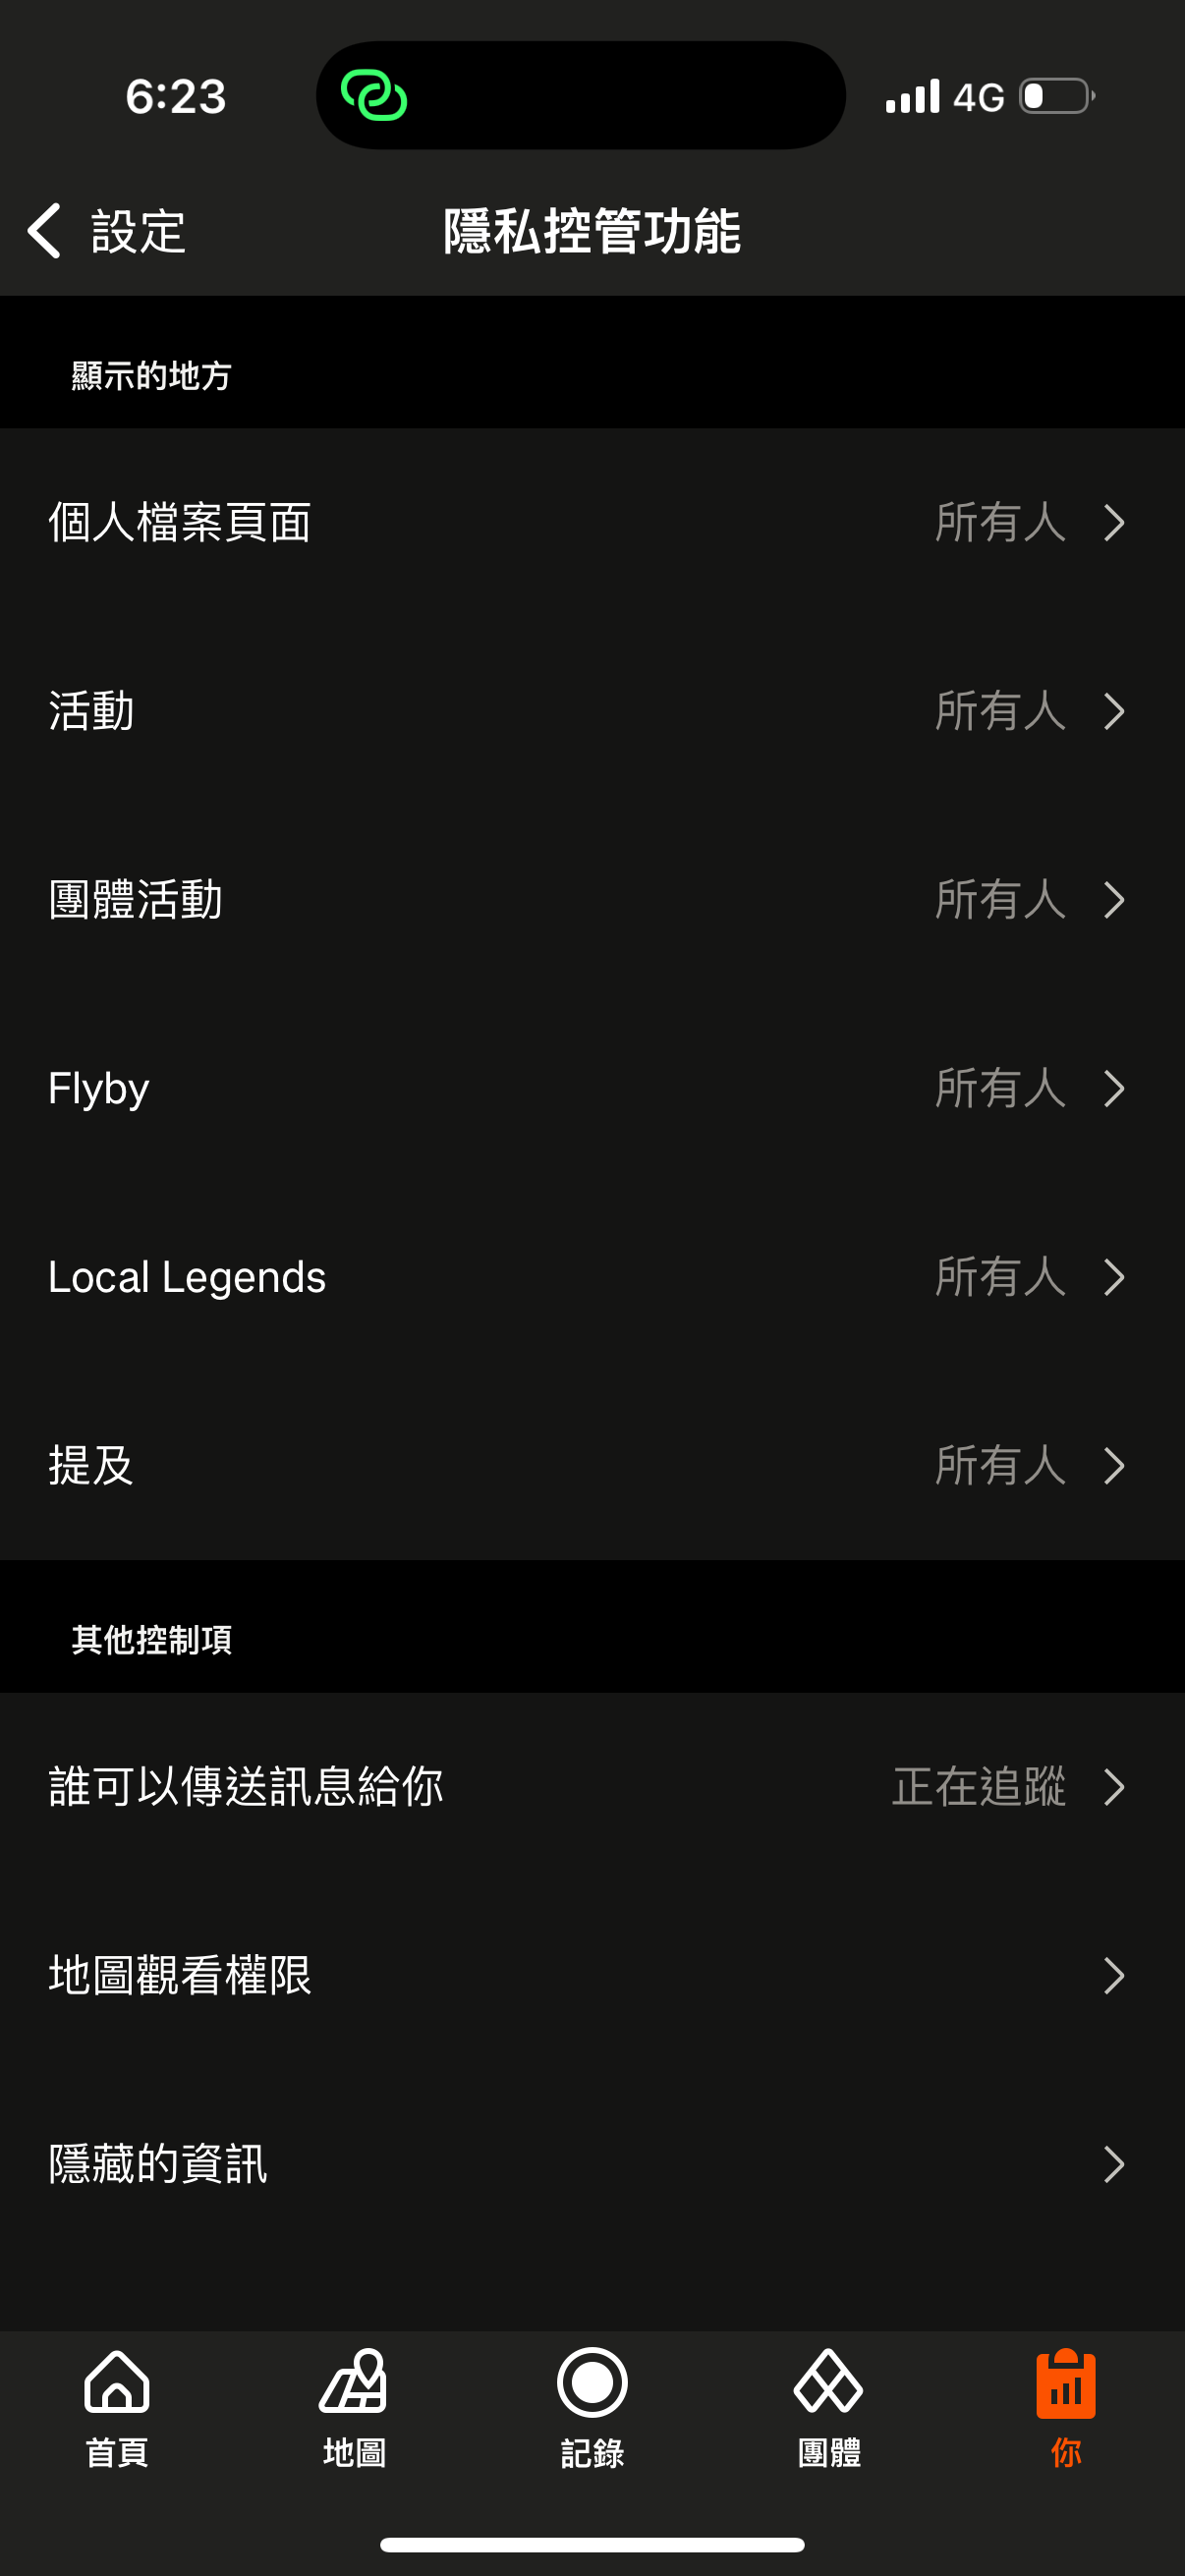
\includegraphics[width=3cm]{privacy.png}
\item 地圖觀看權限\\
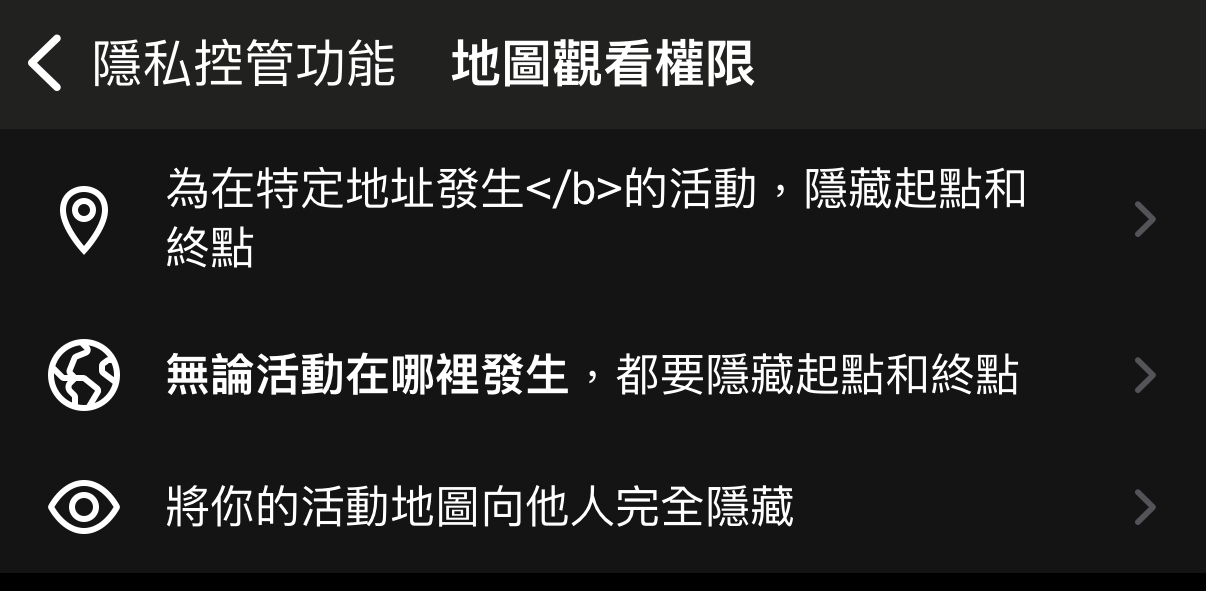
\includegraphics[width=5cm]{hideMap.png}
\end{itemize}
\end{multicols}
\end{frame}

\begin{frame}{騎車人的 Instagram}
\begin{itemize}
\only<1>{
\begin{multicols}{2}
\item 加好友\\

\includegraphics[width=3cm]{friend.png}\\
\item 也可以用搜尋的,但是要把名字放在前面姓氏放在後面搜尋
\newpage
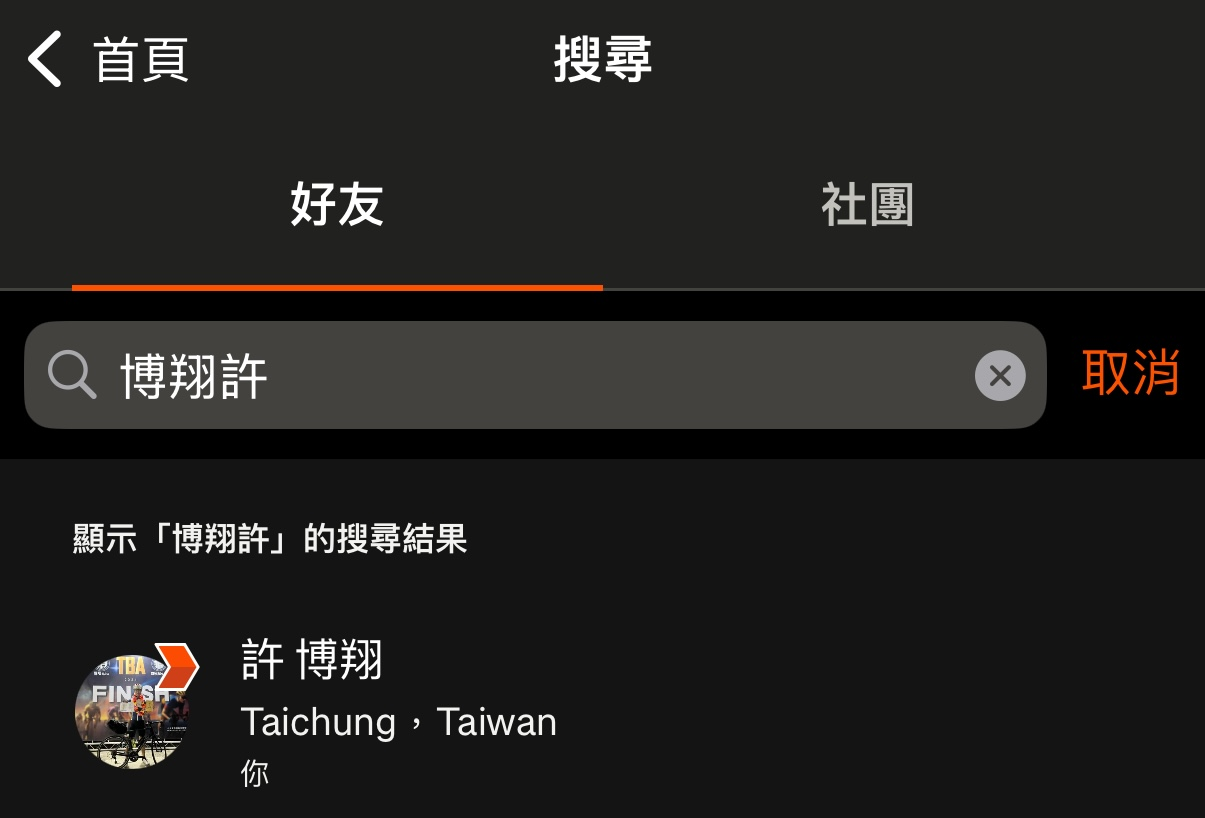
\includegraphics[width=3cm]{search1.png}\\
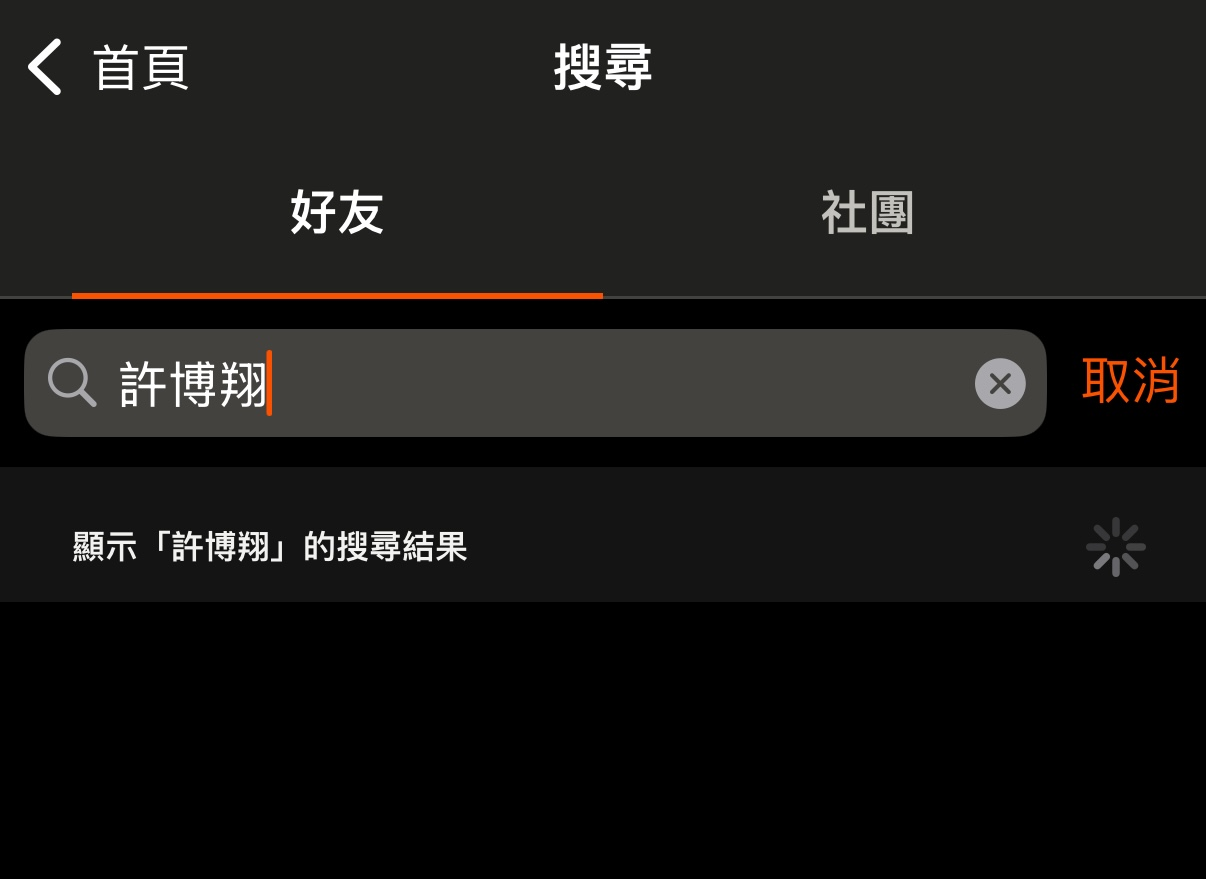
\includegraphics[width=3cm]{search2.png}\\
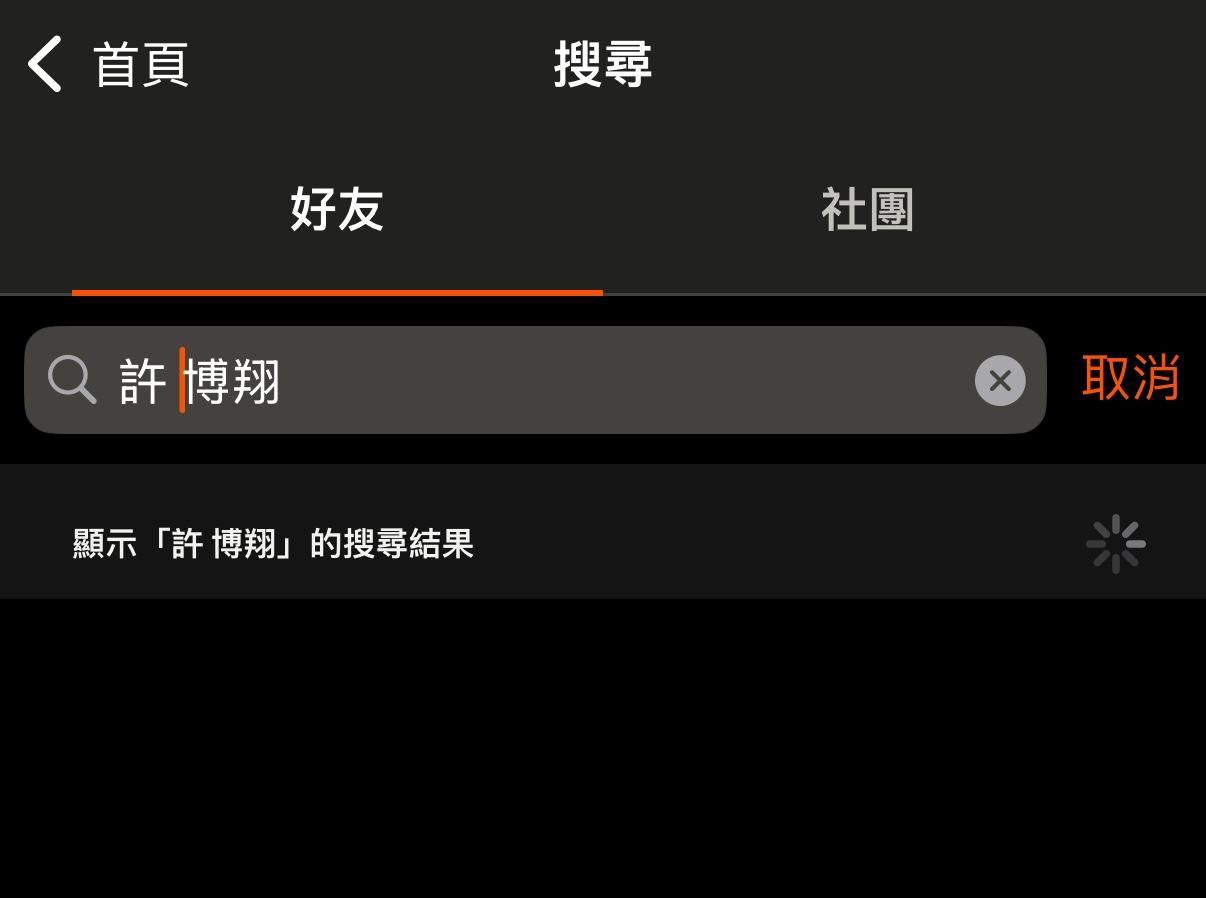
\includegraphics[width=3cm]{search3.png}\\
\end{multicols}
}\only<2>{
\begin{multicols}{2}
\item 加社團\\

\includegraphics[width=3cm]{club.png}
\item 傳訊息\\
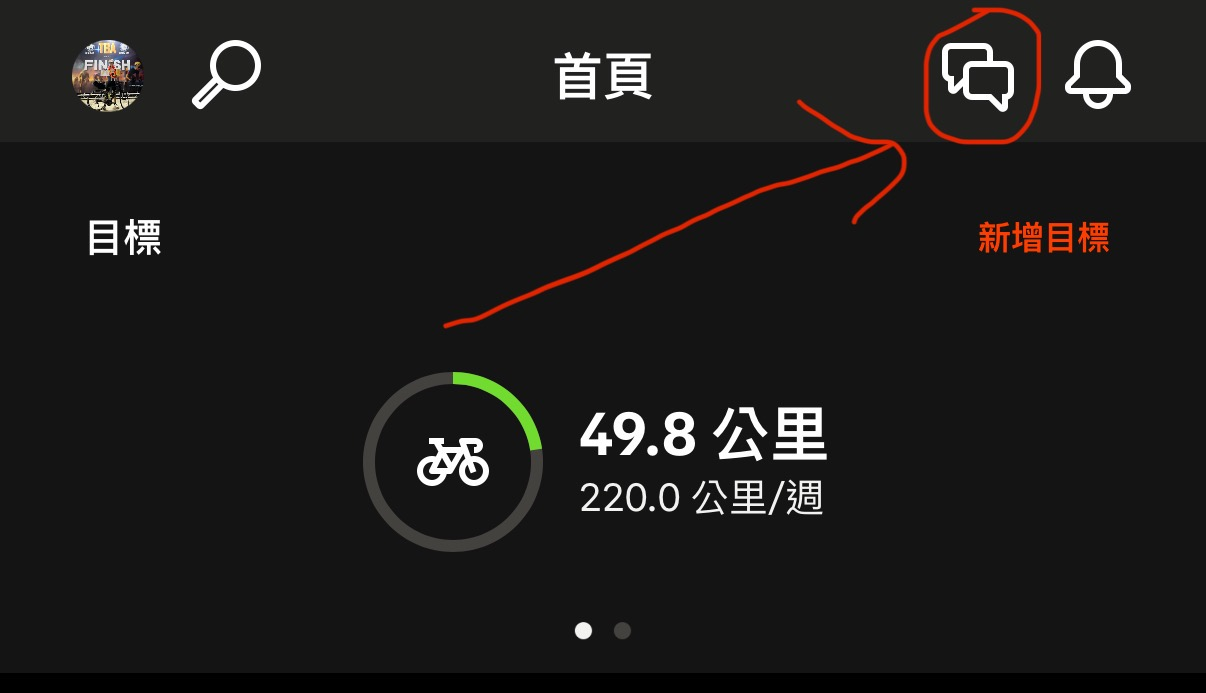
\includegraphics[width=5cm]{message.png}
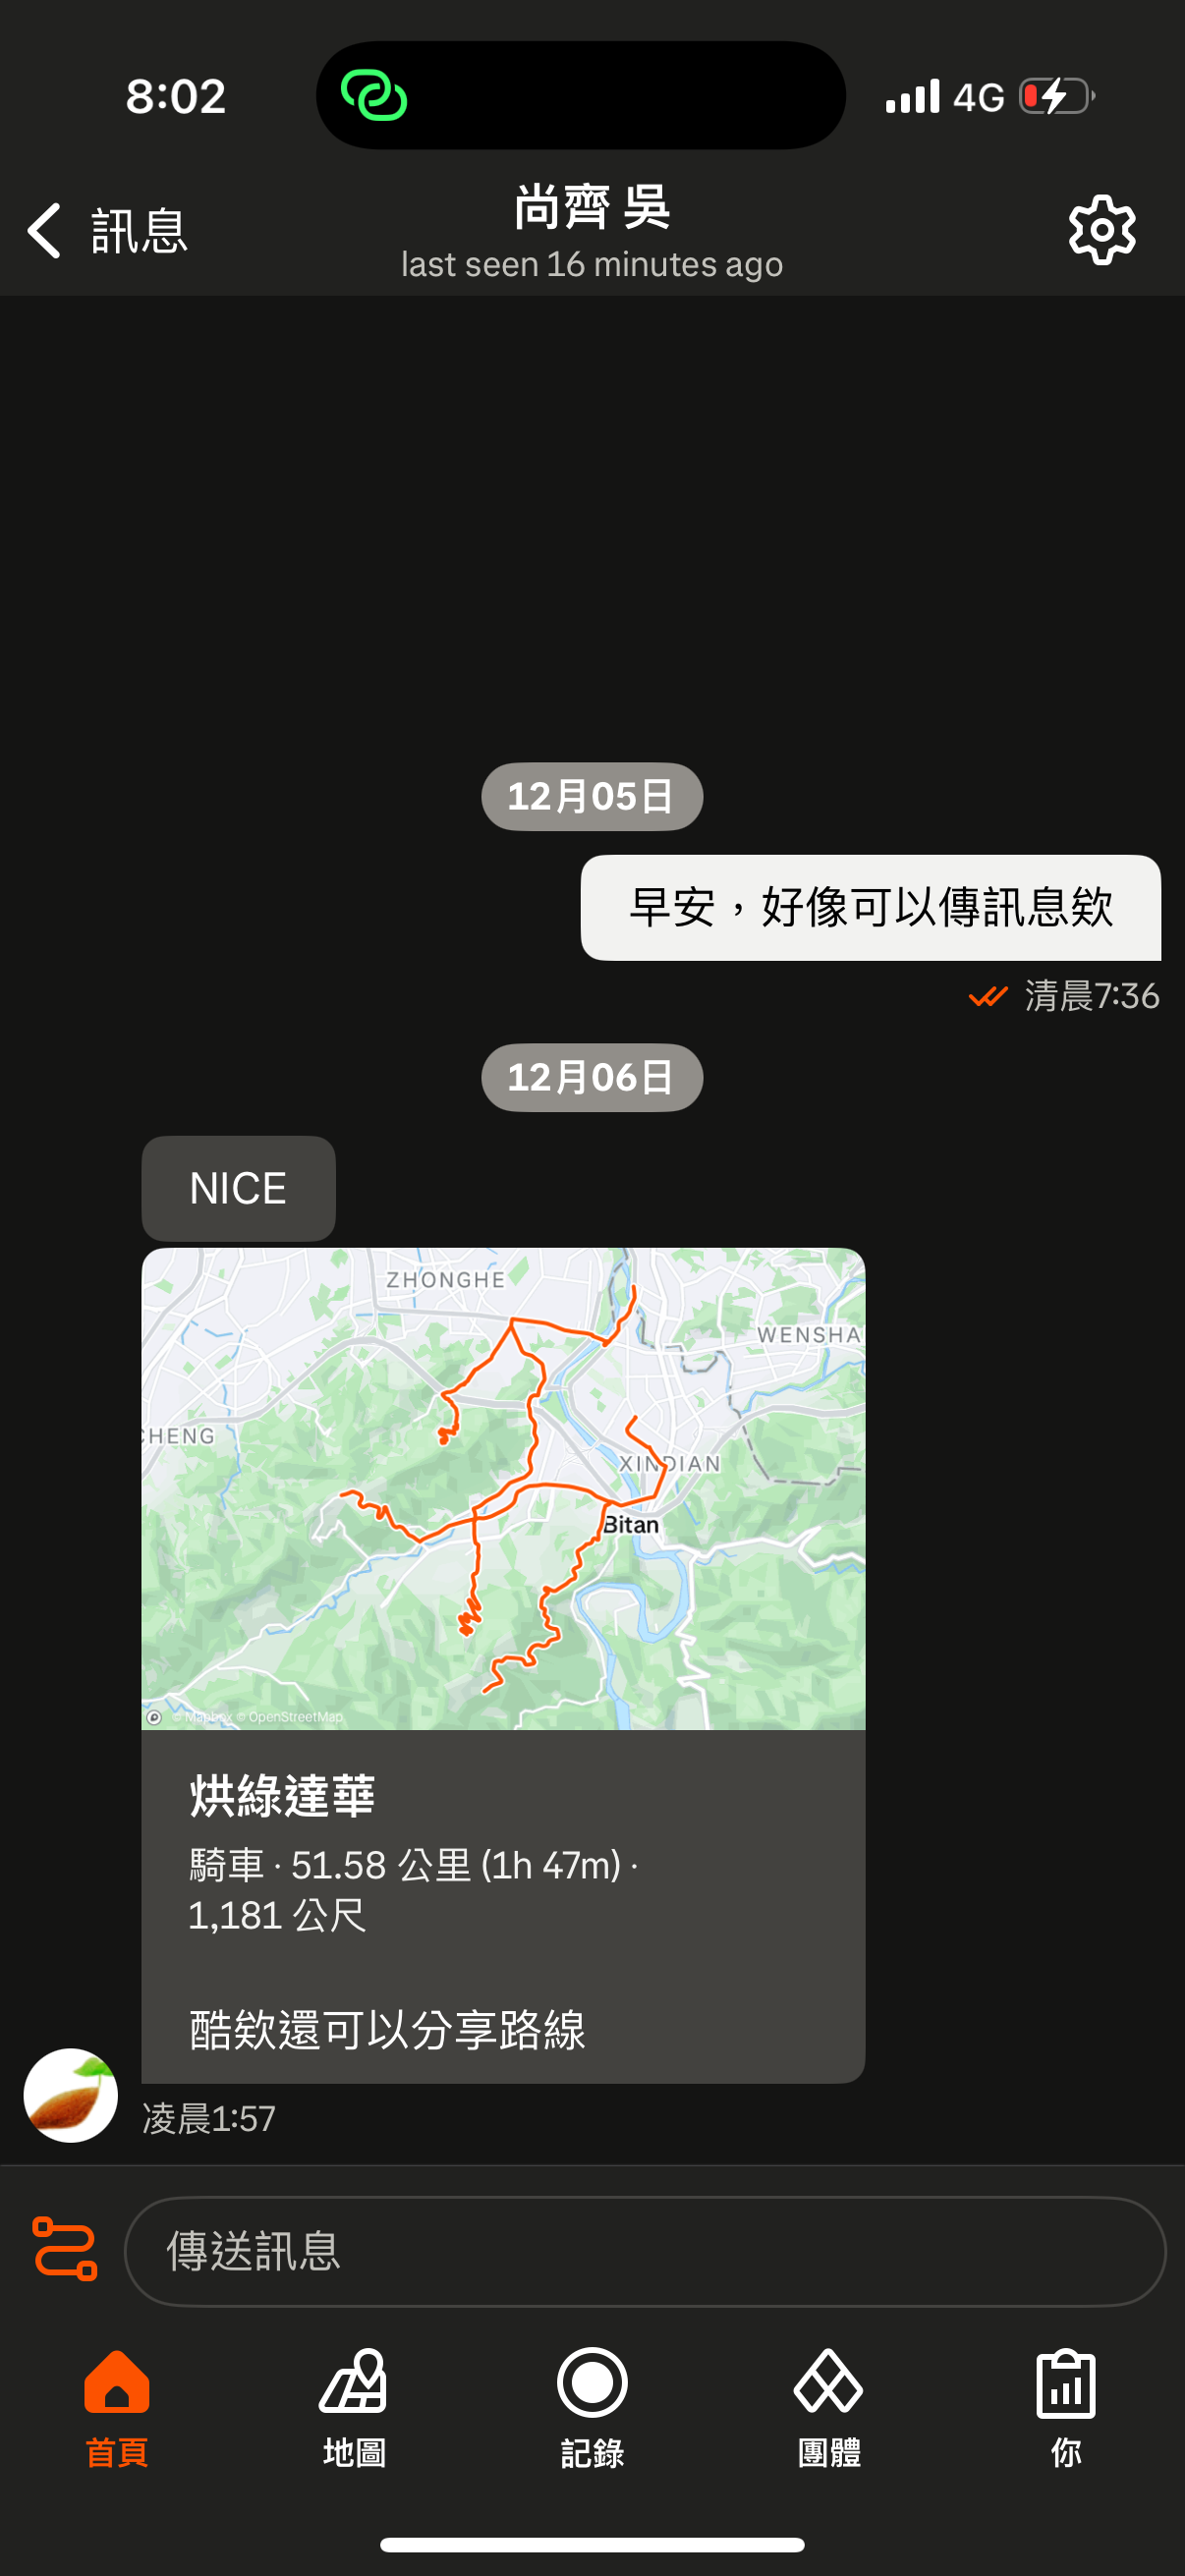
\includegraphics[width=3cm]{message2.png}
\end{multicols}
}\only<3>{
\begin{multicols}{2}
\item 按讚貼文、留言(貼文的讚無法收回,留言的讚可以收回)
\item 貼文、留言都可以標注人
\item 留言無法編輯,但是可以向右滑刪除/檢舉/回覆
\item 自己貼文底下的留言以及自己的留言可以刪除
\item 別人的留言可以檢舉/回覆
\newpage
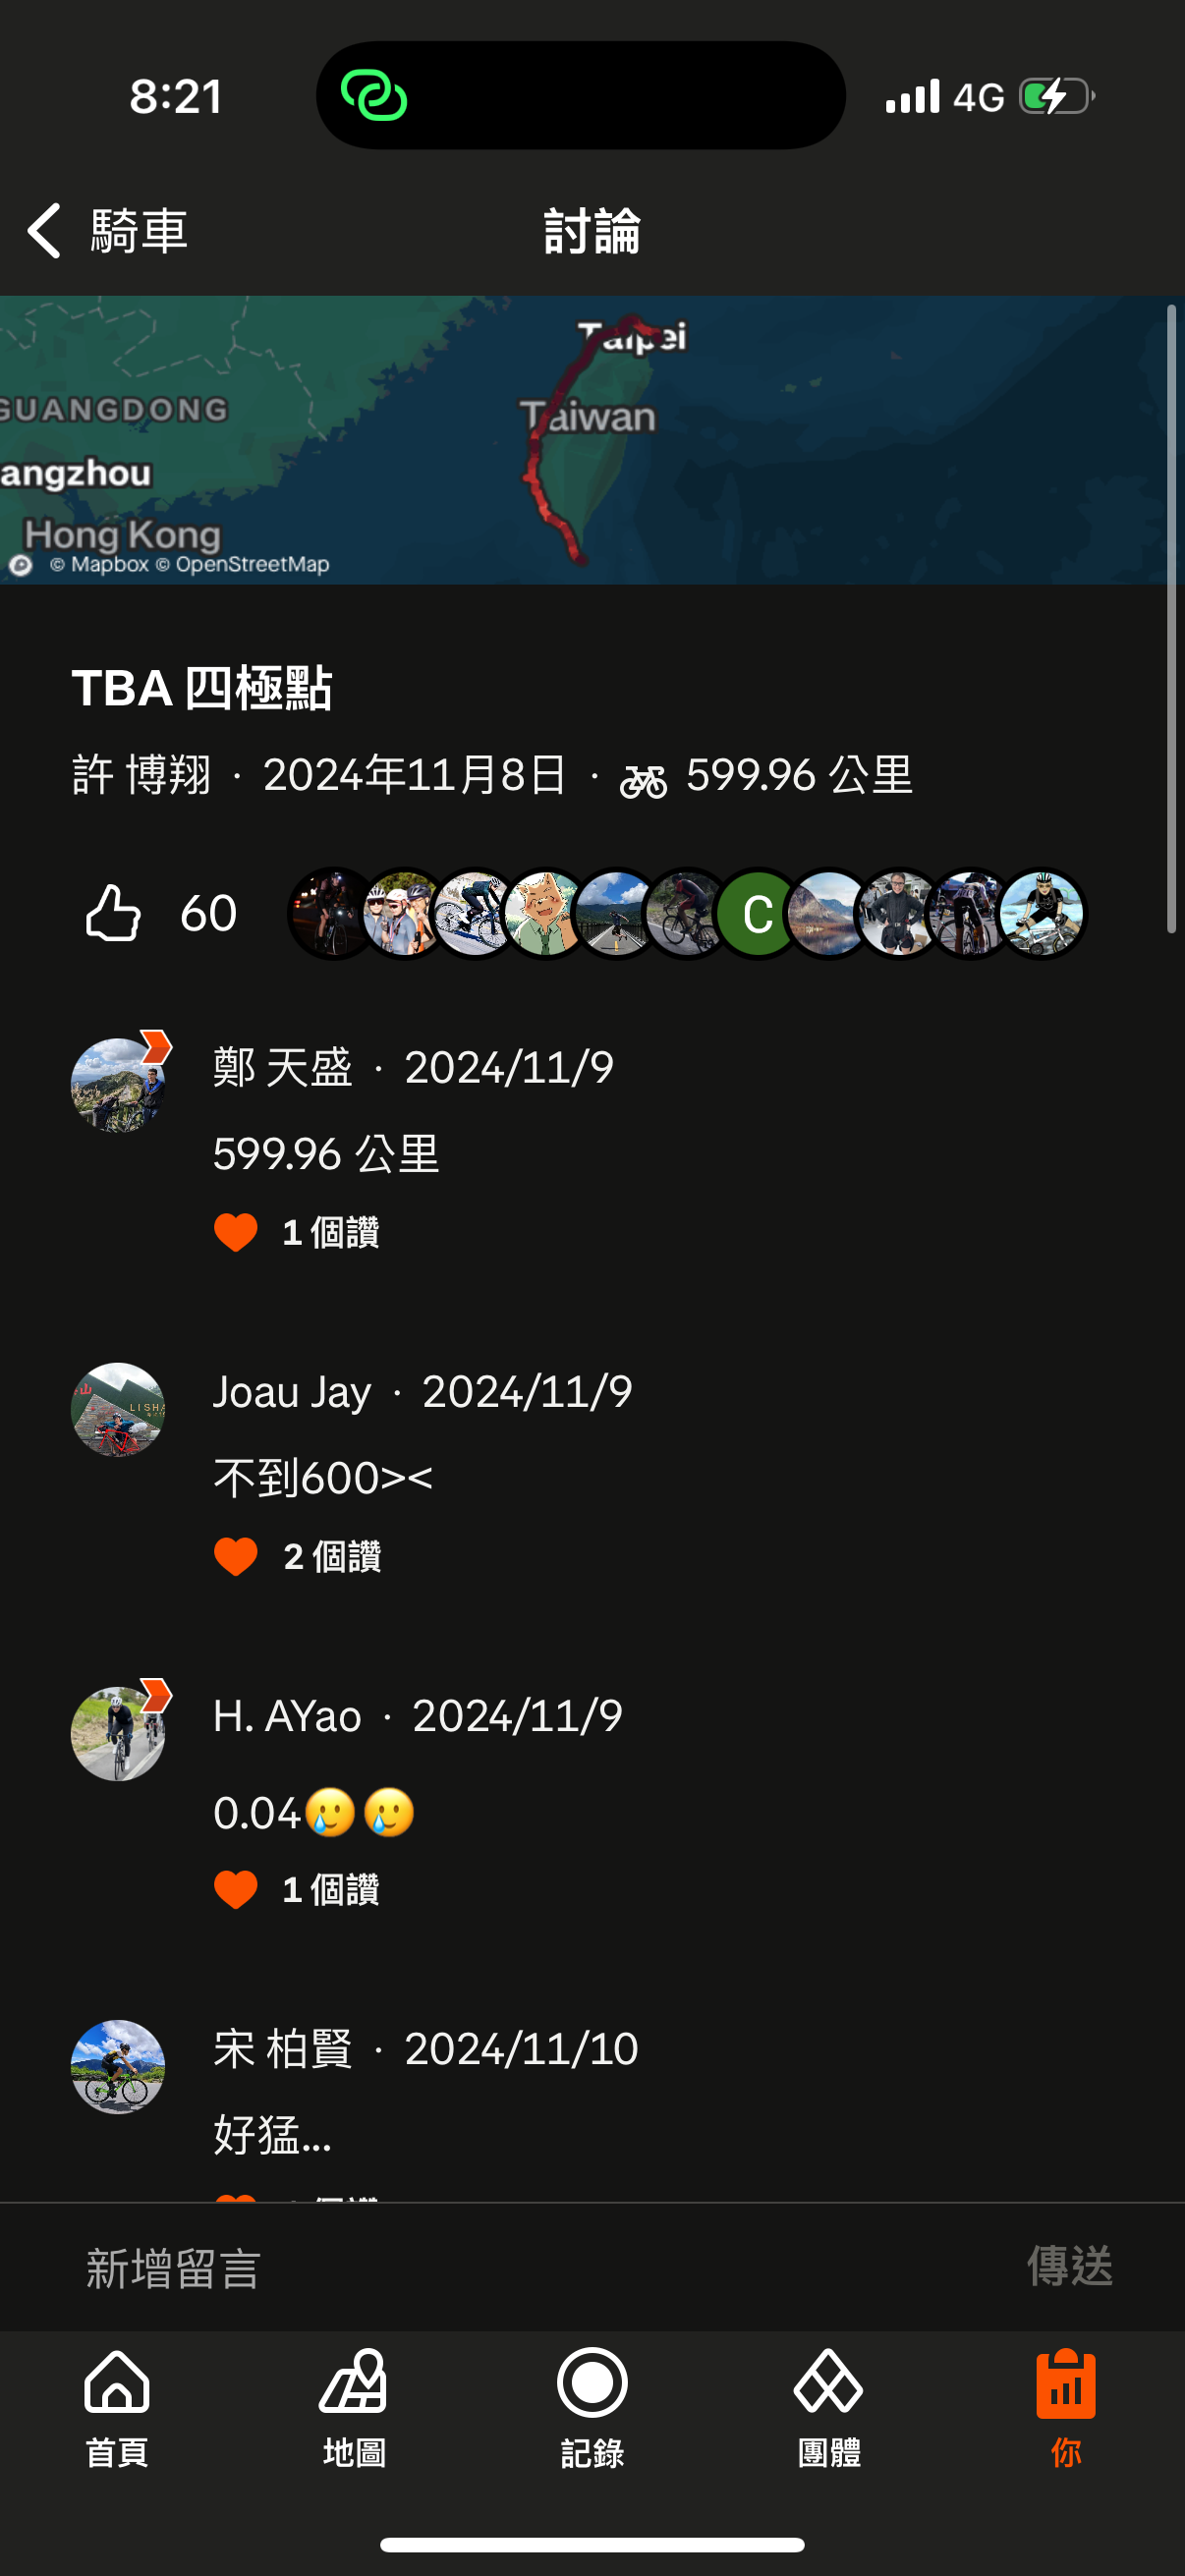
\includegraphics[width=3cm]{post.png}
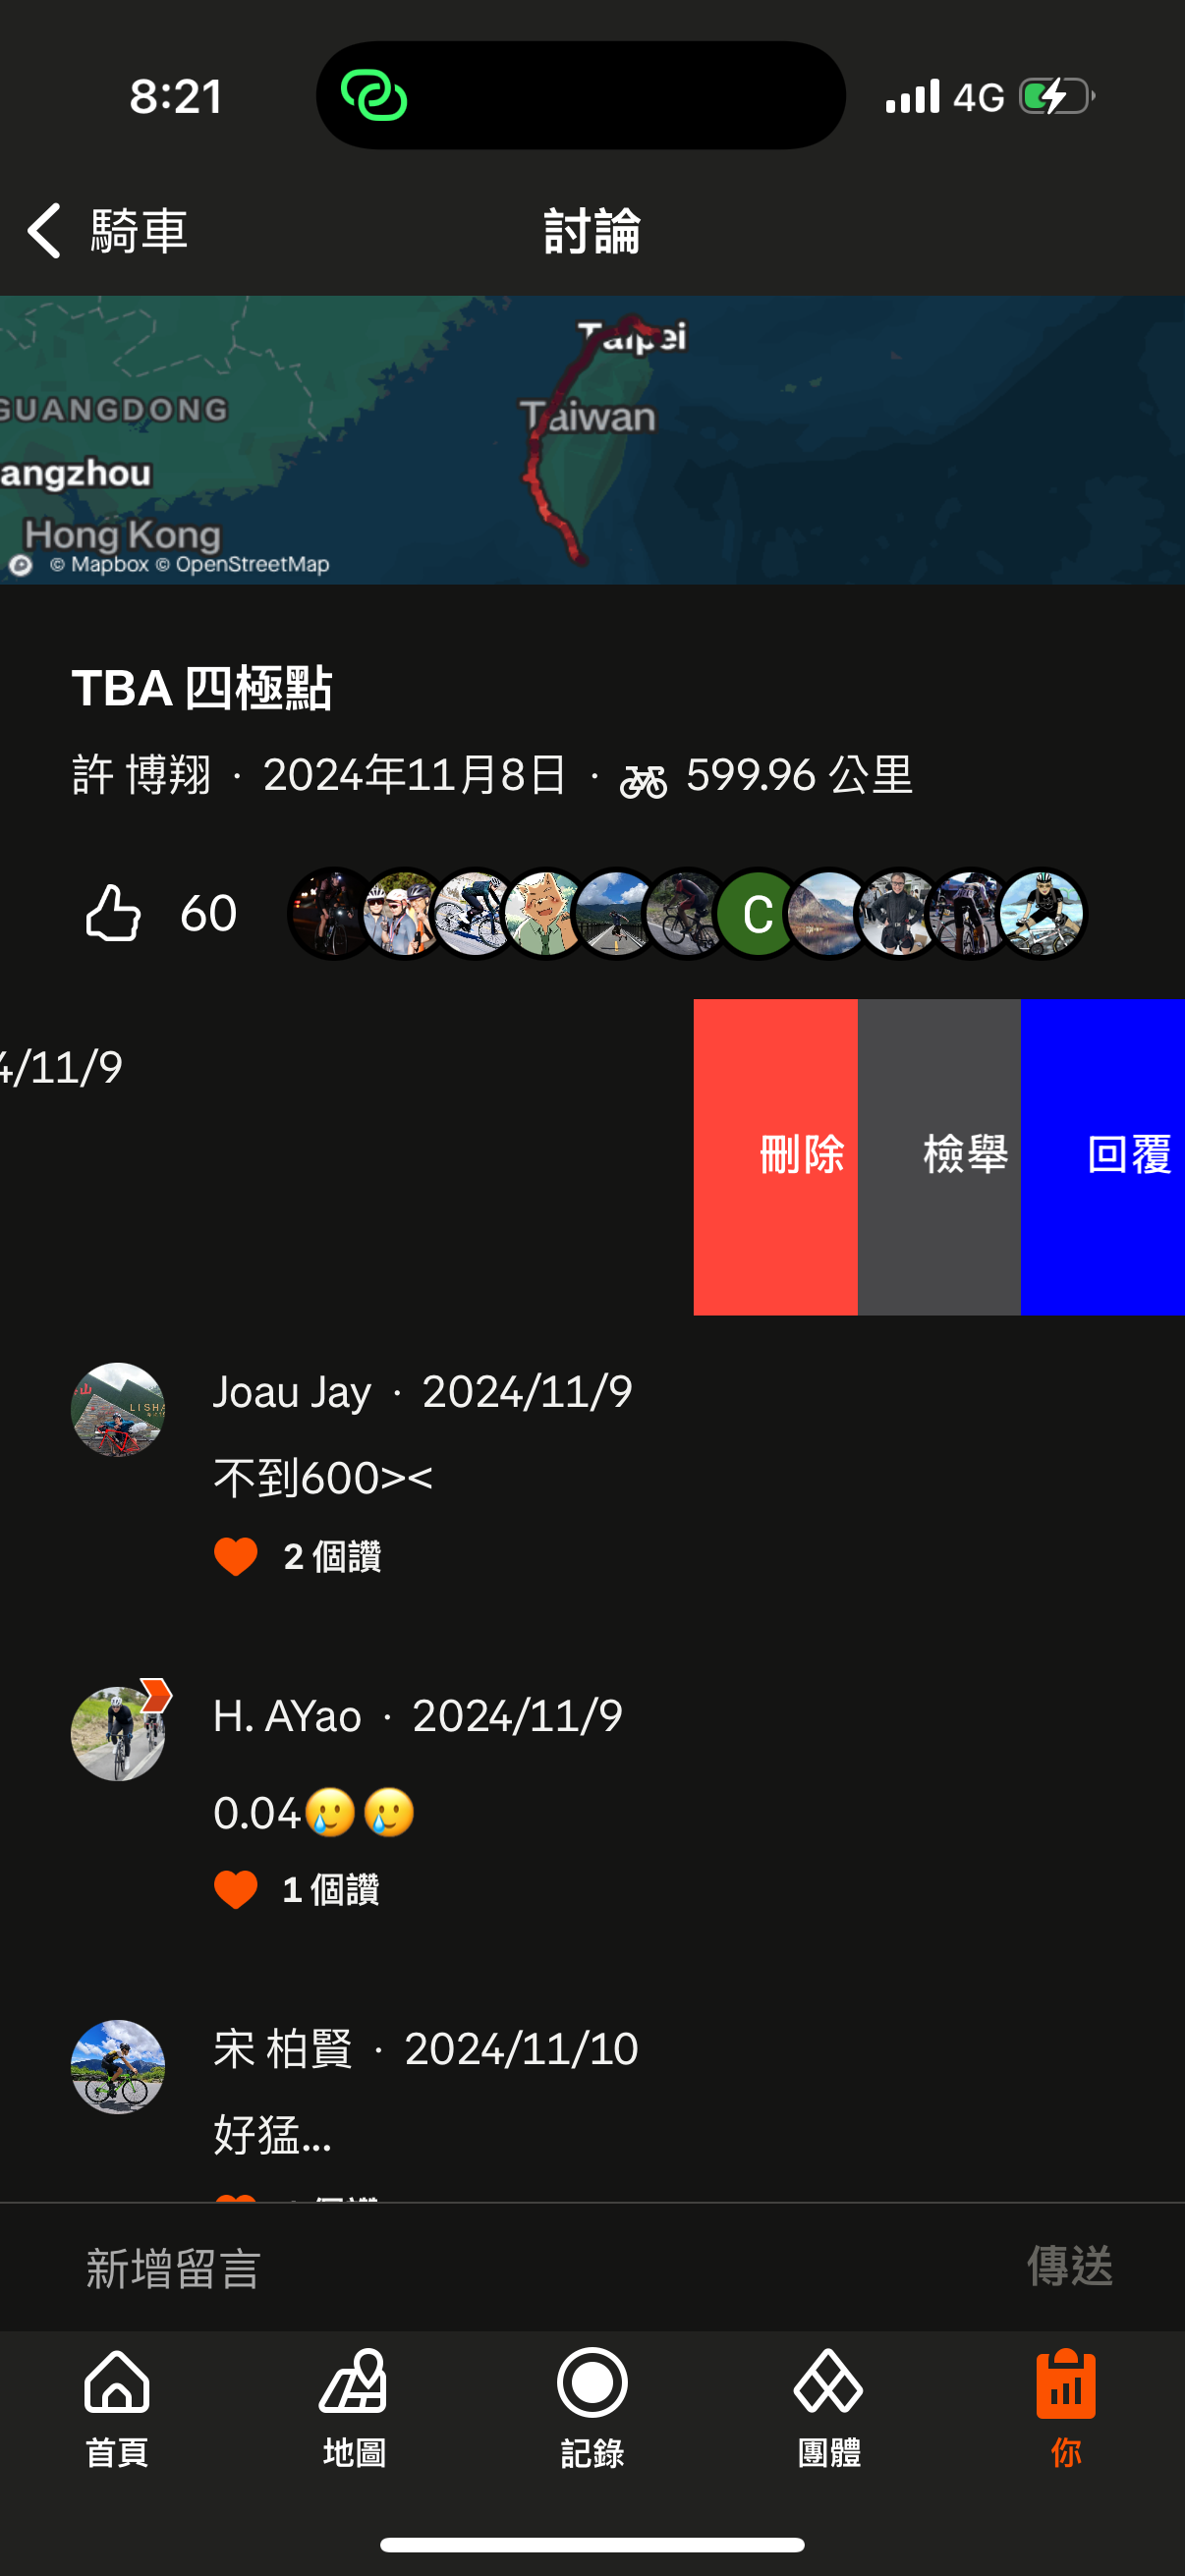
\includegraphics[width=3cm]{post2.png}
\end{multicols}
}\only<4->{
\pause\pause\pause
\item \begin{center}\begin{tabular}{c|c}
Strava & Instagram\\\hline\pause
可以加好友 & 可以加好友\\\pause
可以加社團 & 可以加社團\\\pause
可以傳訊息 & 可以傳訊息\\\pause
可以發文 & 可以發文\\\pause
貼文可以放照片 & 貼文可以放照片\\\pause
可以留言 & 可以留言\\\pause
可以按讚貼文/留言 & 可以按讚貼文/留言\\\pause
可以刪除貼文/留言 & 可以刪除貼文/留言\\\pause
可以放地圖 & 不能放地圖\\\pause
可以刷路段 & 不能刷路段\\\pause
可以計算運動的數據 & 無法計算運動的數據\\\pause
不會被祖 & 可能會被祖
\end{tabular}\end{center}
}
\end{itemize}
\end{frame}

\begin{frame}{騎車人的 Instagram}
\only<1-3>{
\begin{itemize}
\item 
\includegraphics[width=5cm]{happen.png}
\pause
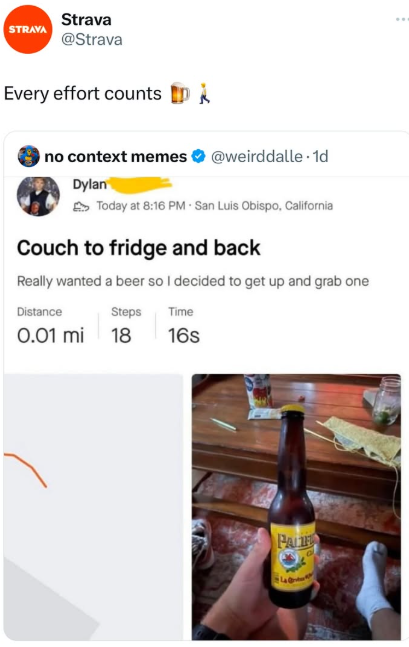
\includegraphics[width=3cm]{everyEffortCounts.png}
\pause
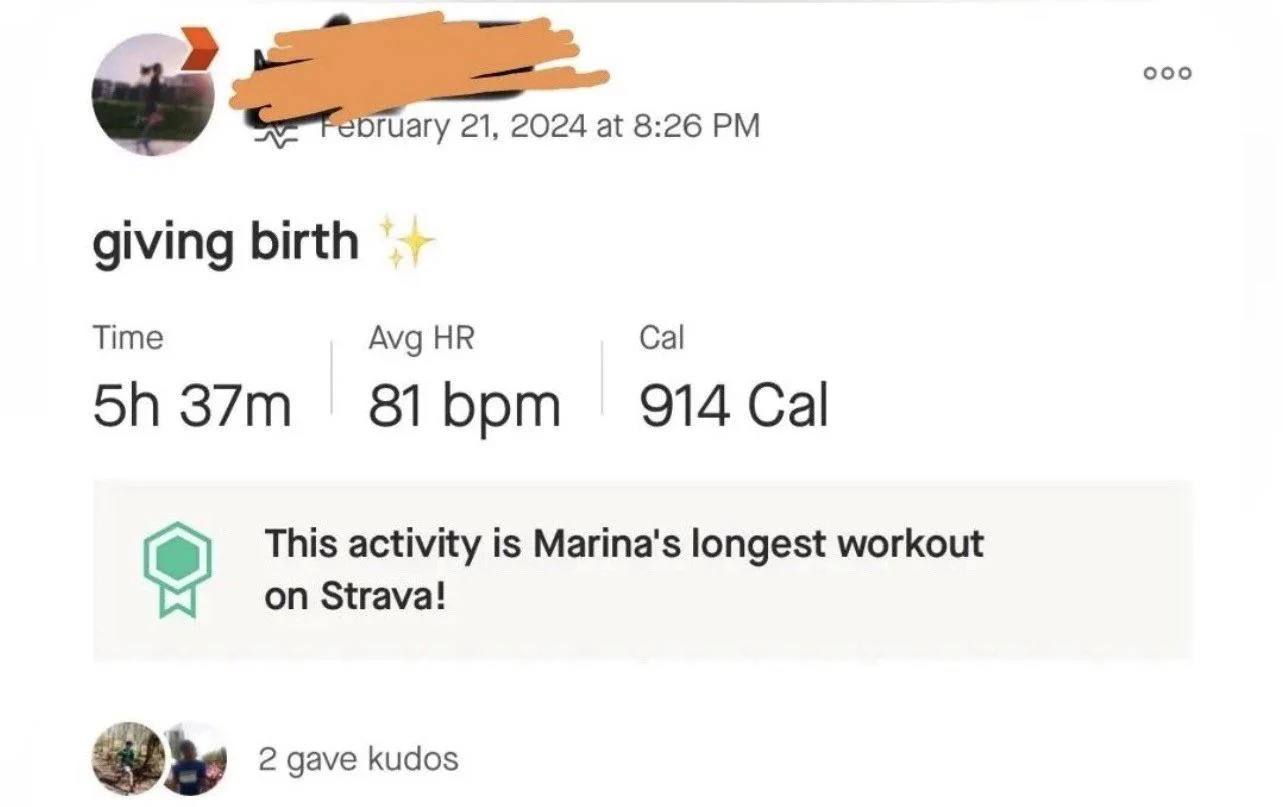
\includegraphics[width=6cm]{giveBirth.png}
\end{itemize}
}\only<4-5>{
\pause\pause\pause
\begin{itemize}
\begin{multicols}{2}
\item 
\includegraphics[width=5cm]{forgetResume.jpeg}
\pause
\item \href{https://www.instagram.com/jonagraphs/reel/C-G-Cf_R5c6/}{When the run doesn't save.}
\item 
\includegraphics[width=5cm]{saveWhenCrash.jpg}
\end{multicols}
\end{itemize}
}\only<6->{
\pause\pause\pause\pause\pause
\begin{itemize}
\item 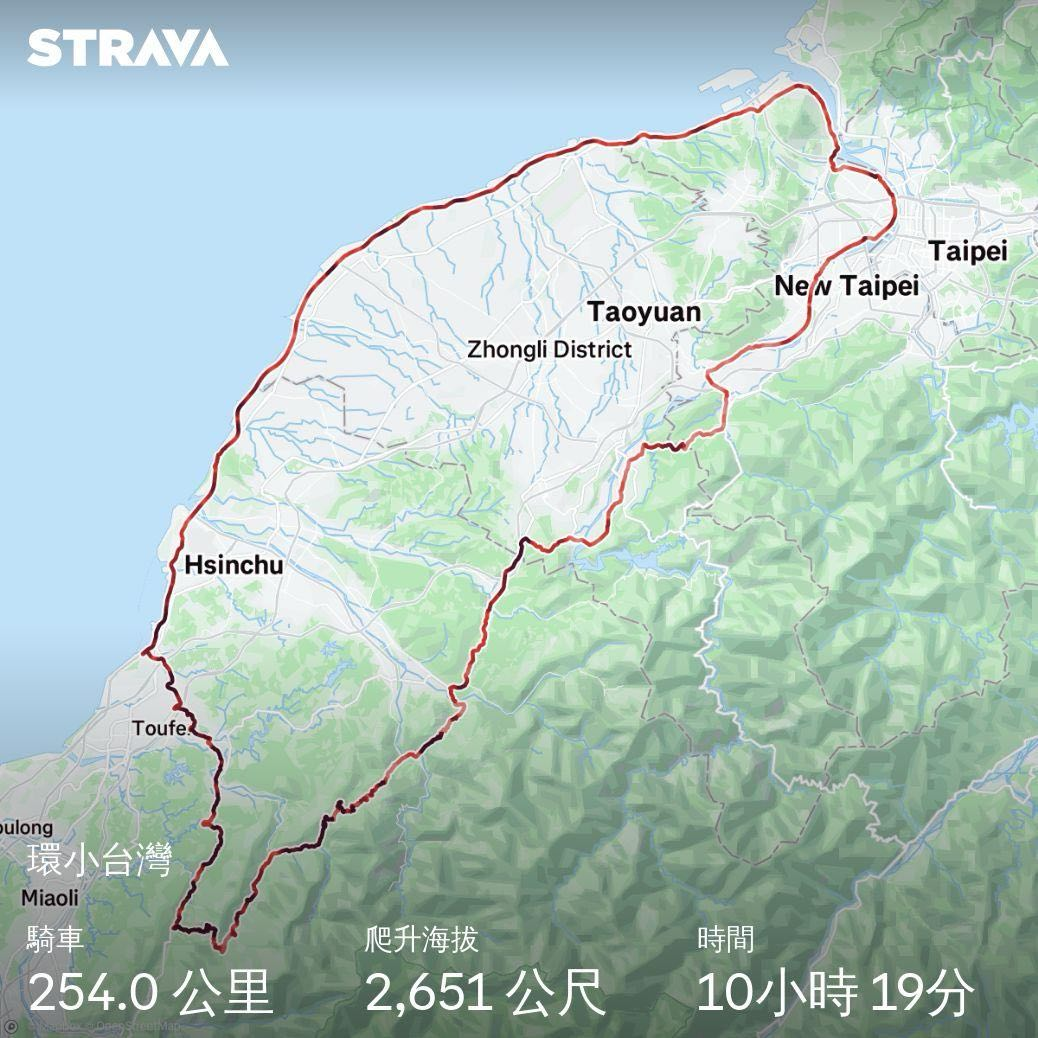
\includegraphics[height=3.5cm]{smallTaiwan.jpg}\pause
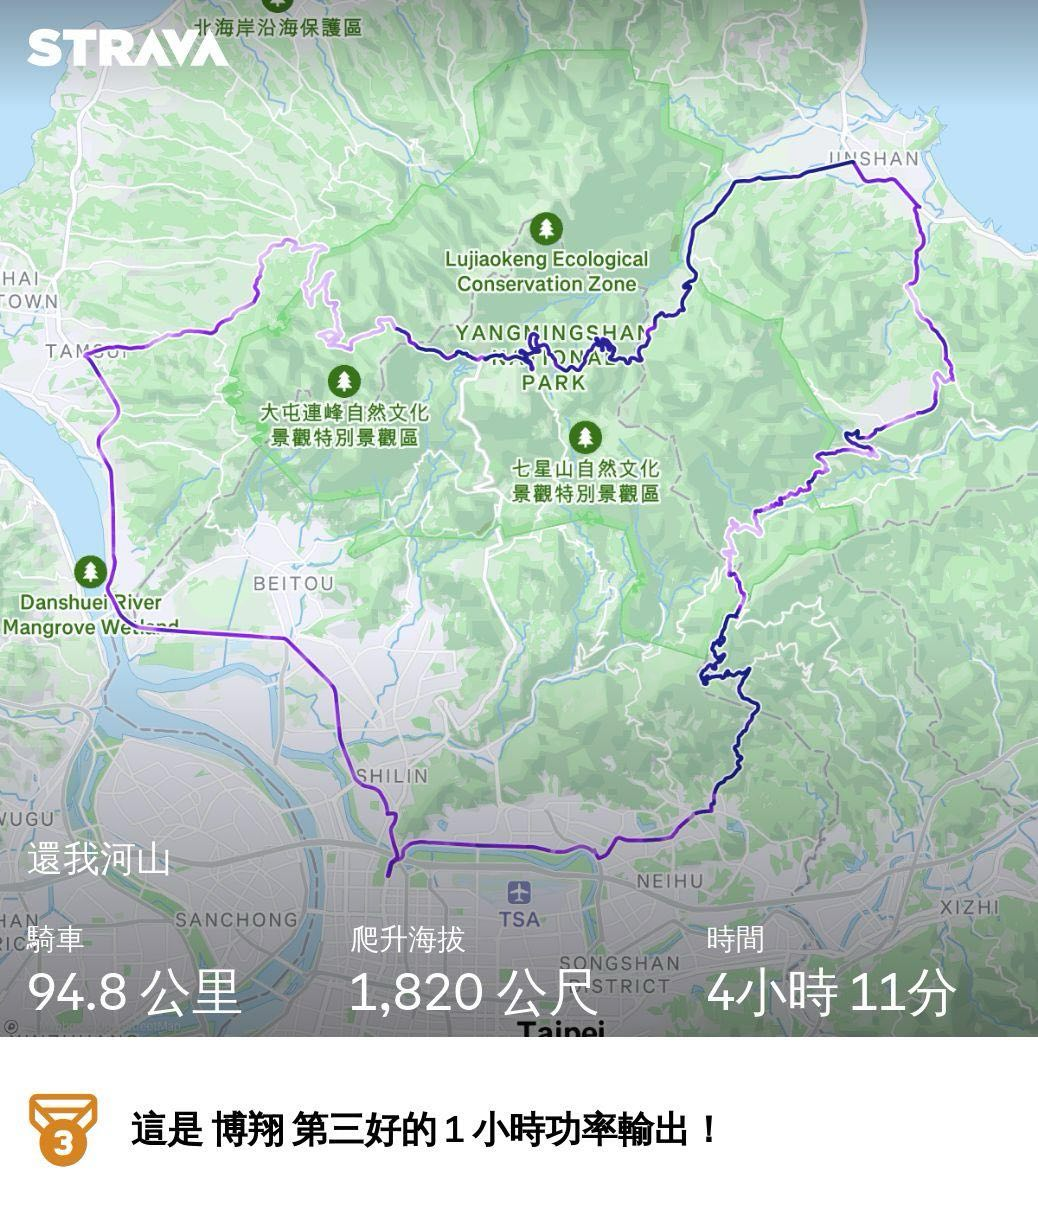
\includegraphics[height=3.5cm]{china.jpg}\pause
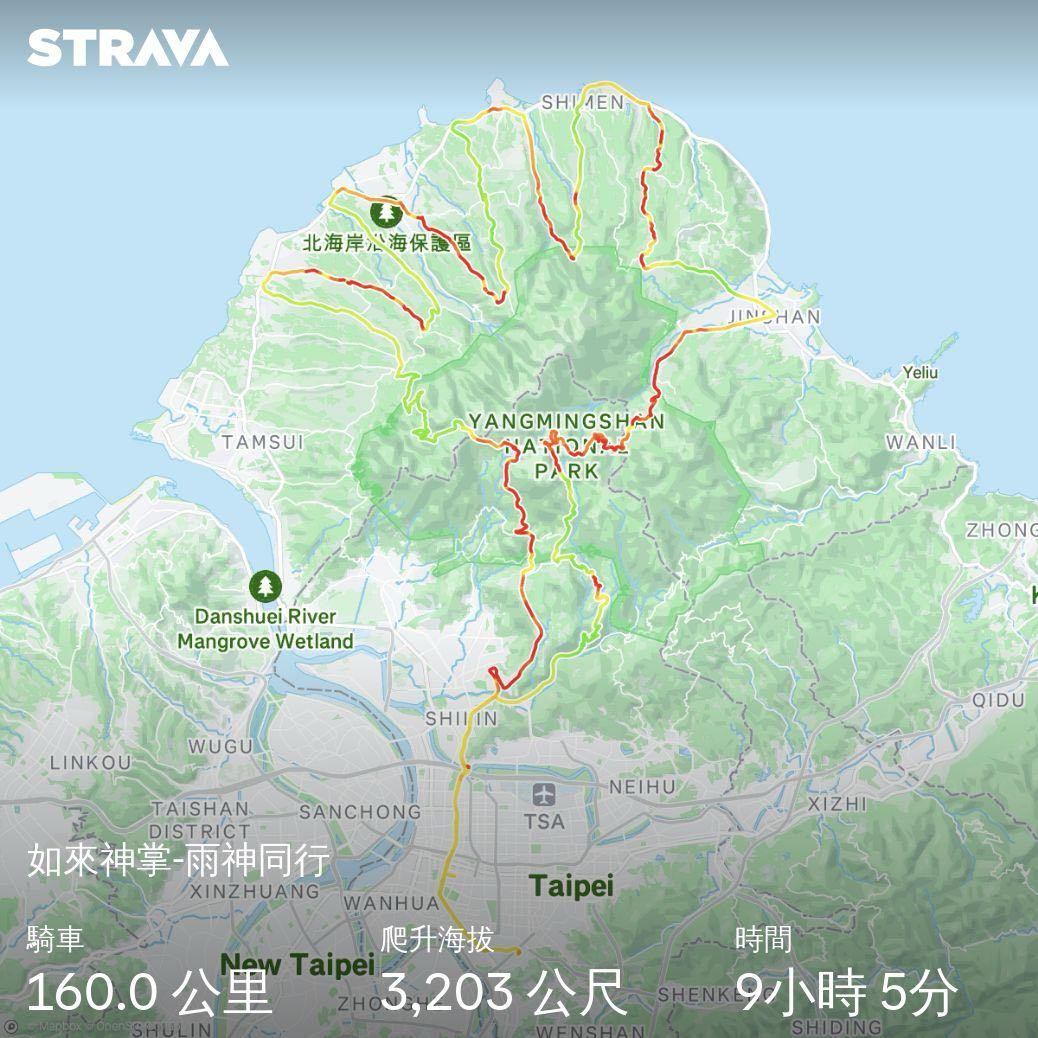
\includegraphics[height=3.5cm]{paw.jpg}\pause
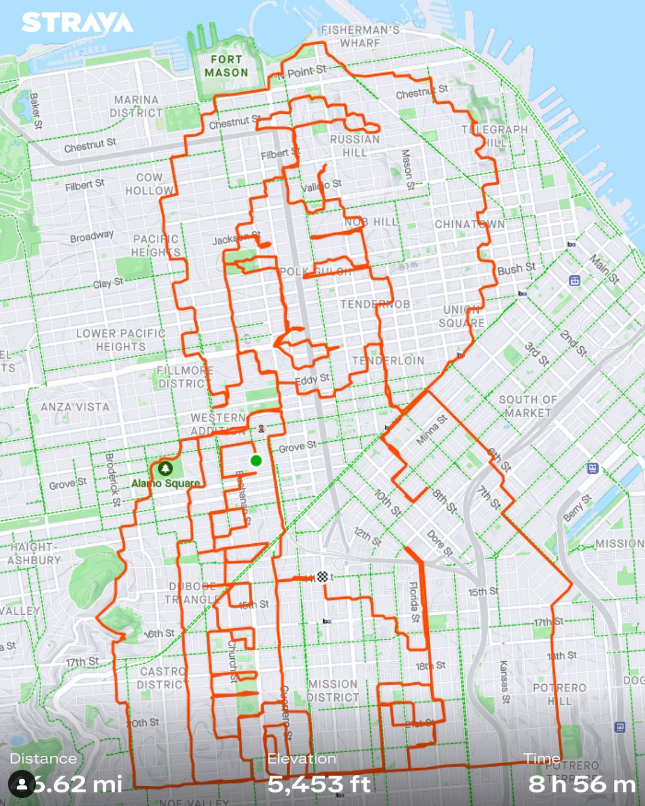
\includegraphics[height=3.5cm]{woman.png}\\\pause
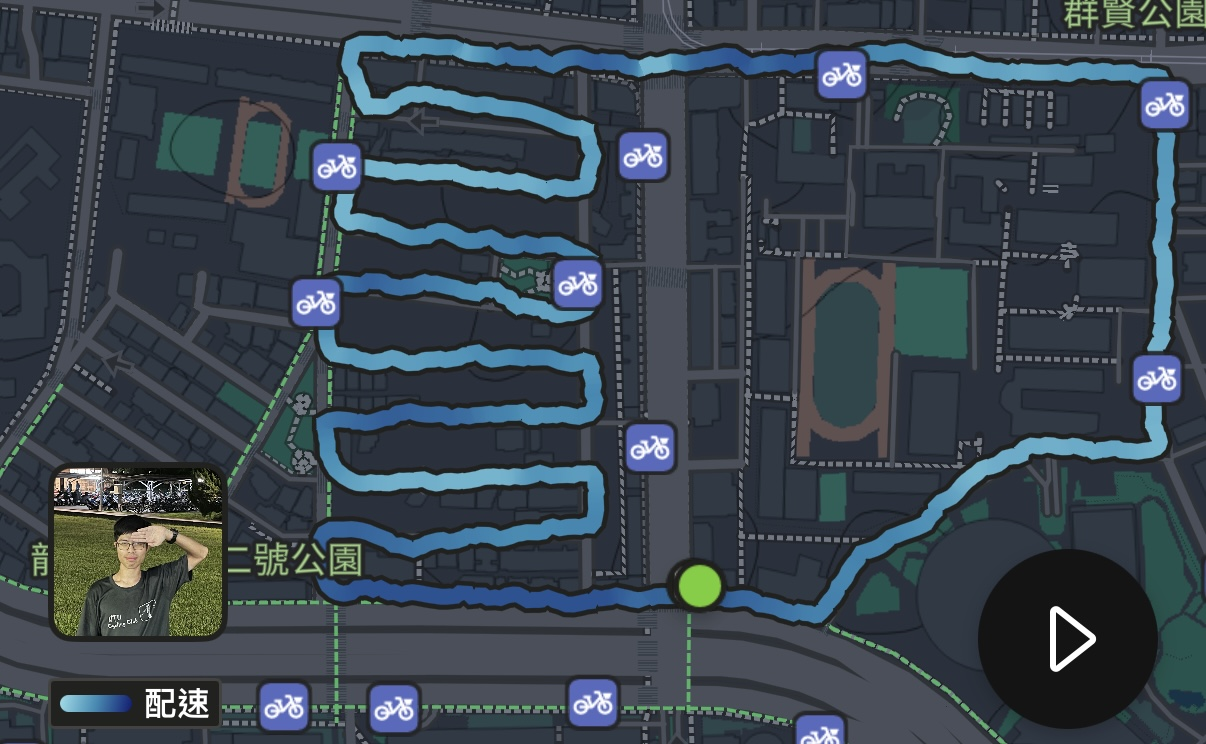
\includegraphics[height=3cm]{118.png}\pause
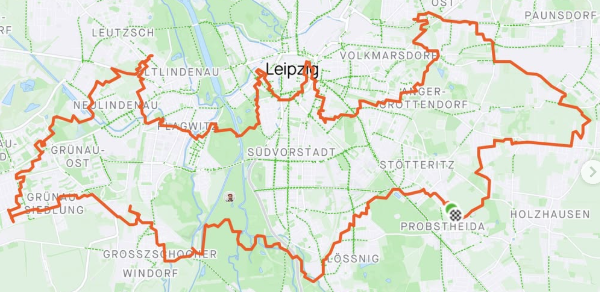
\includegraphics[height=3cm]{batman.png}\pause
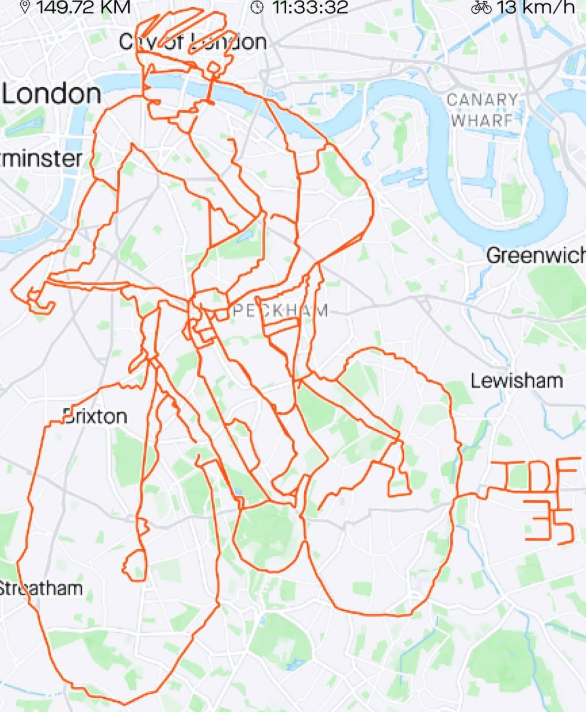
\includegraphics[height=3cm]{cyclist.png}\pause
\item \href{https://www.instagram.com/p/DCy7qa_NzUl/}{You can even dance on map.}
\end{itemize}
}
\end{frame}

\begin{frame}{團體活動}
\begin{multicols}{2}
\begin{itemize}
\item 忘了紀錄活動或是紀錄有問題怎麼辦?請一起運動的朋友標注你\\
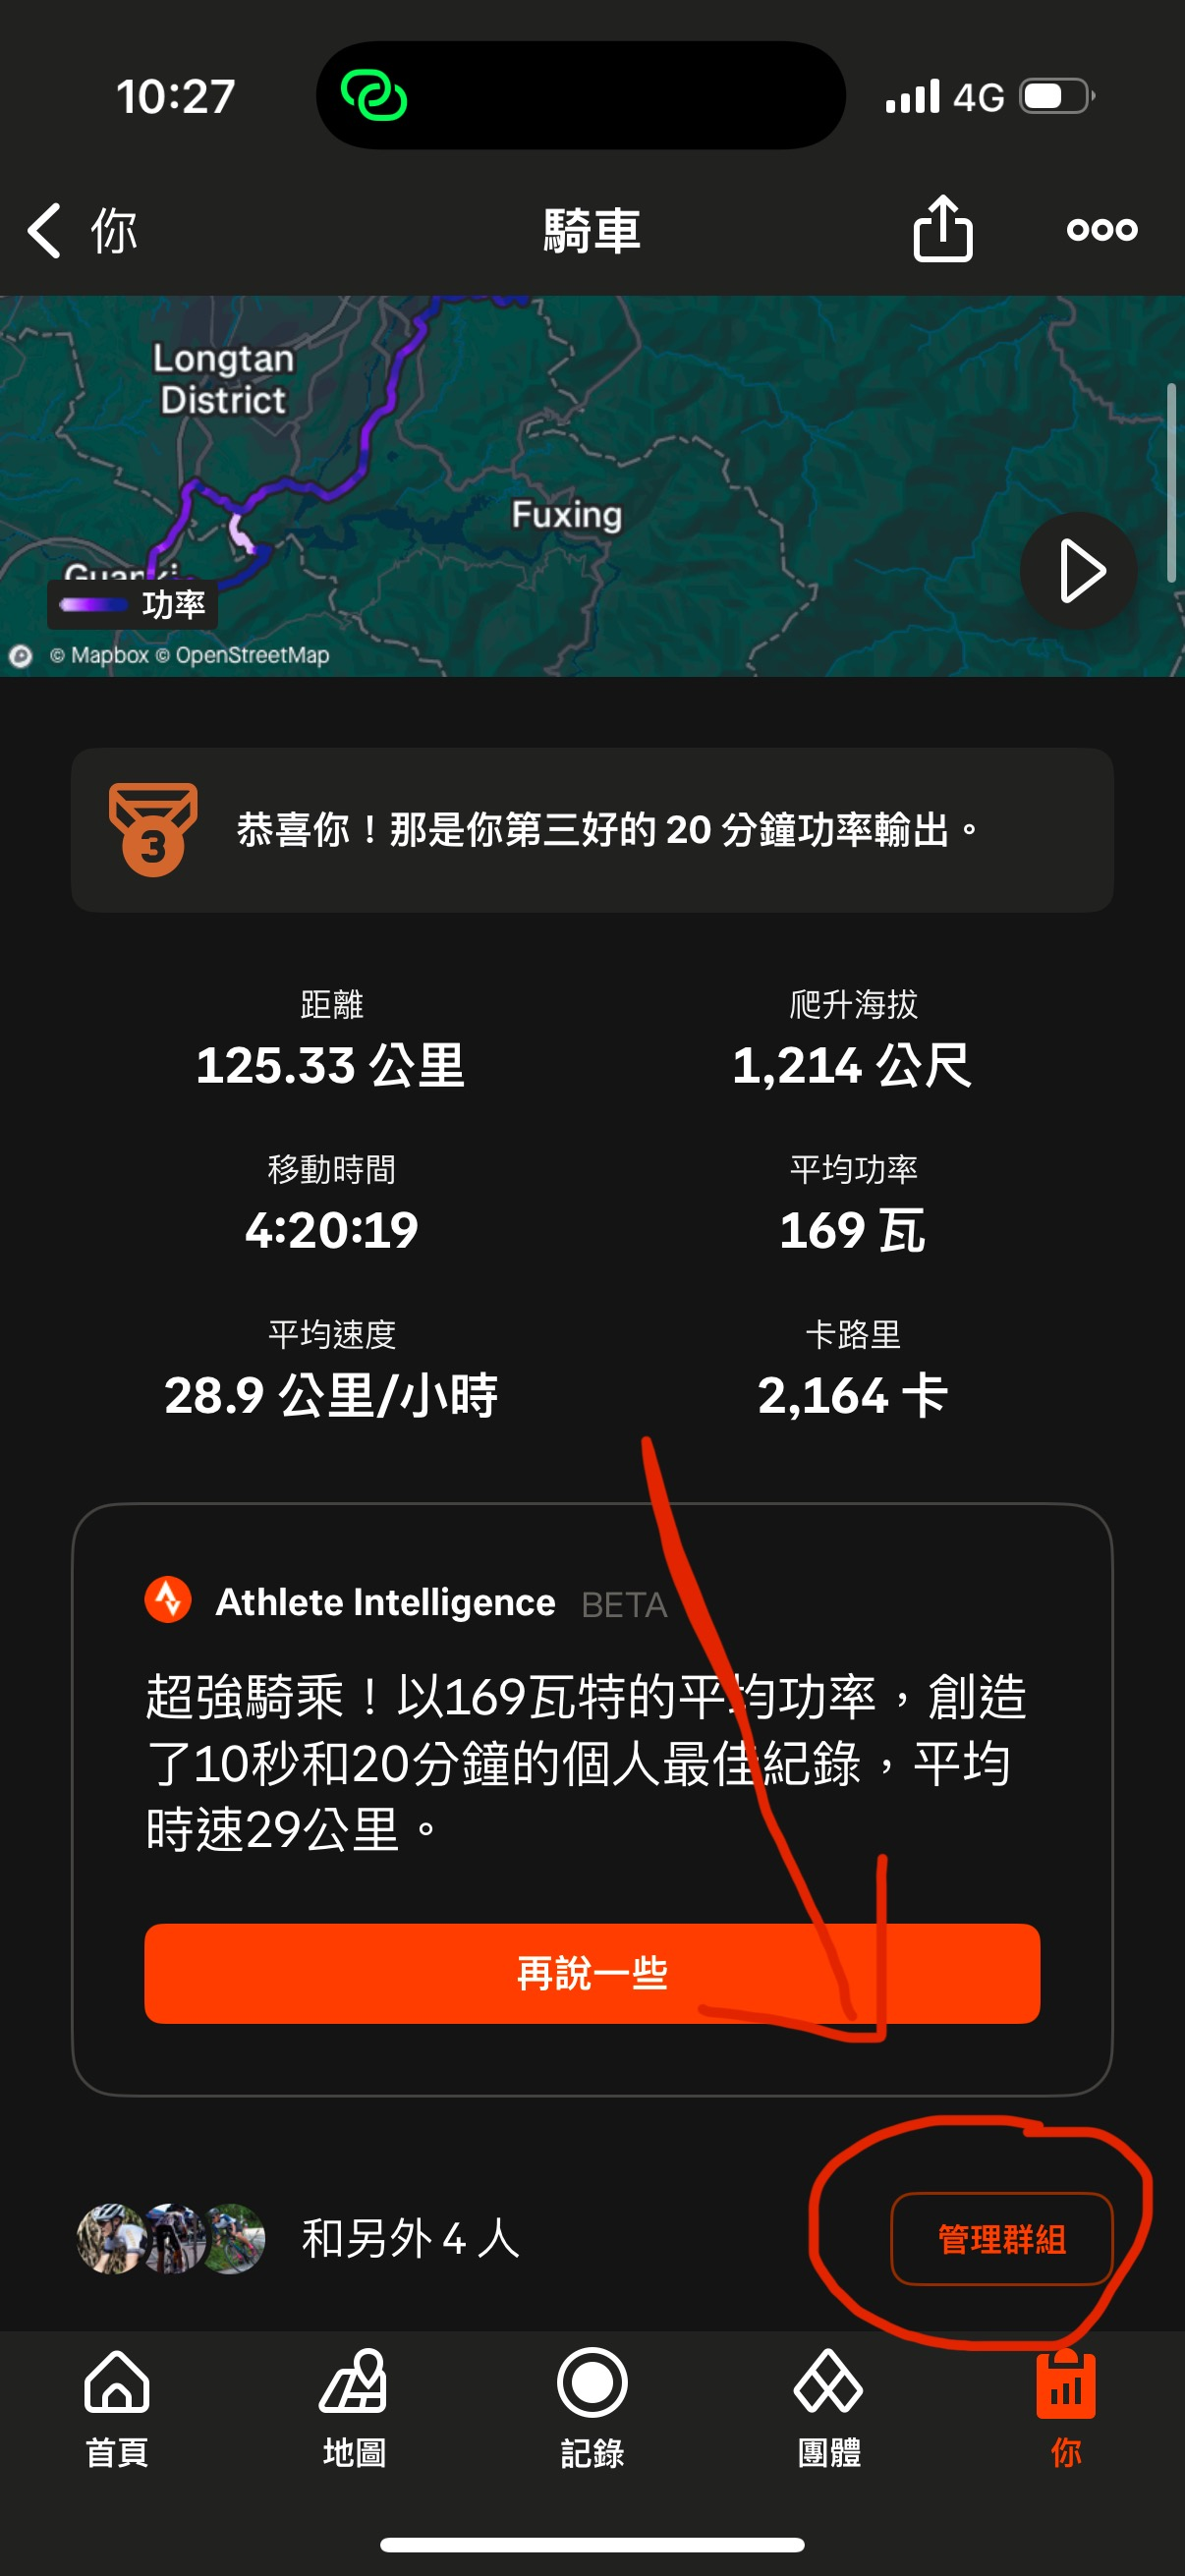
\includegraphics[width=3cm]{rideTogether.png}
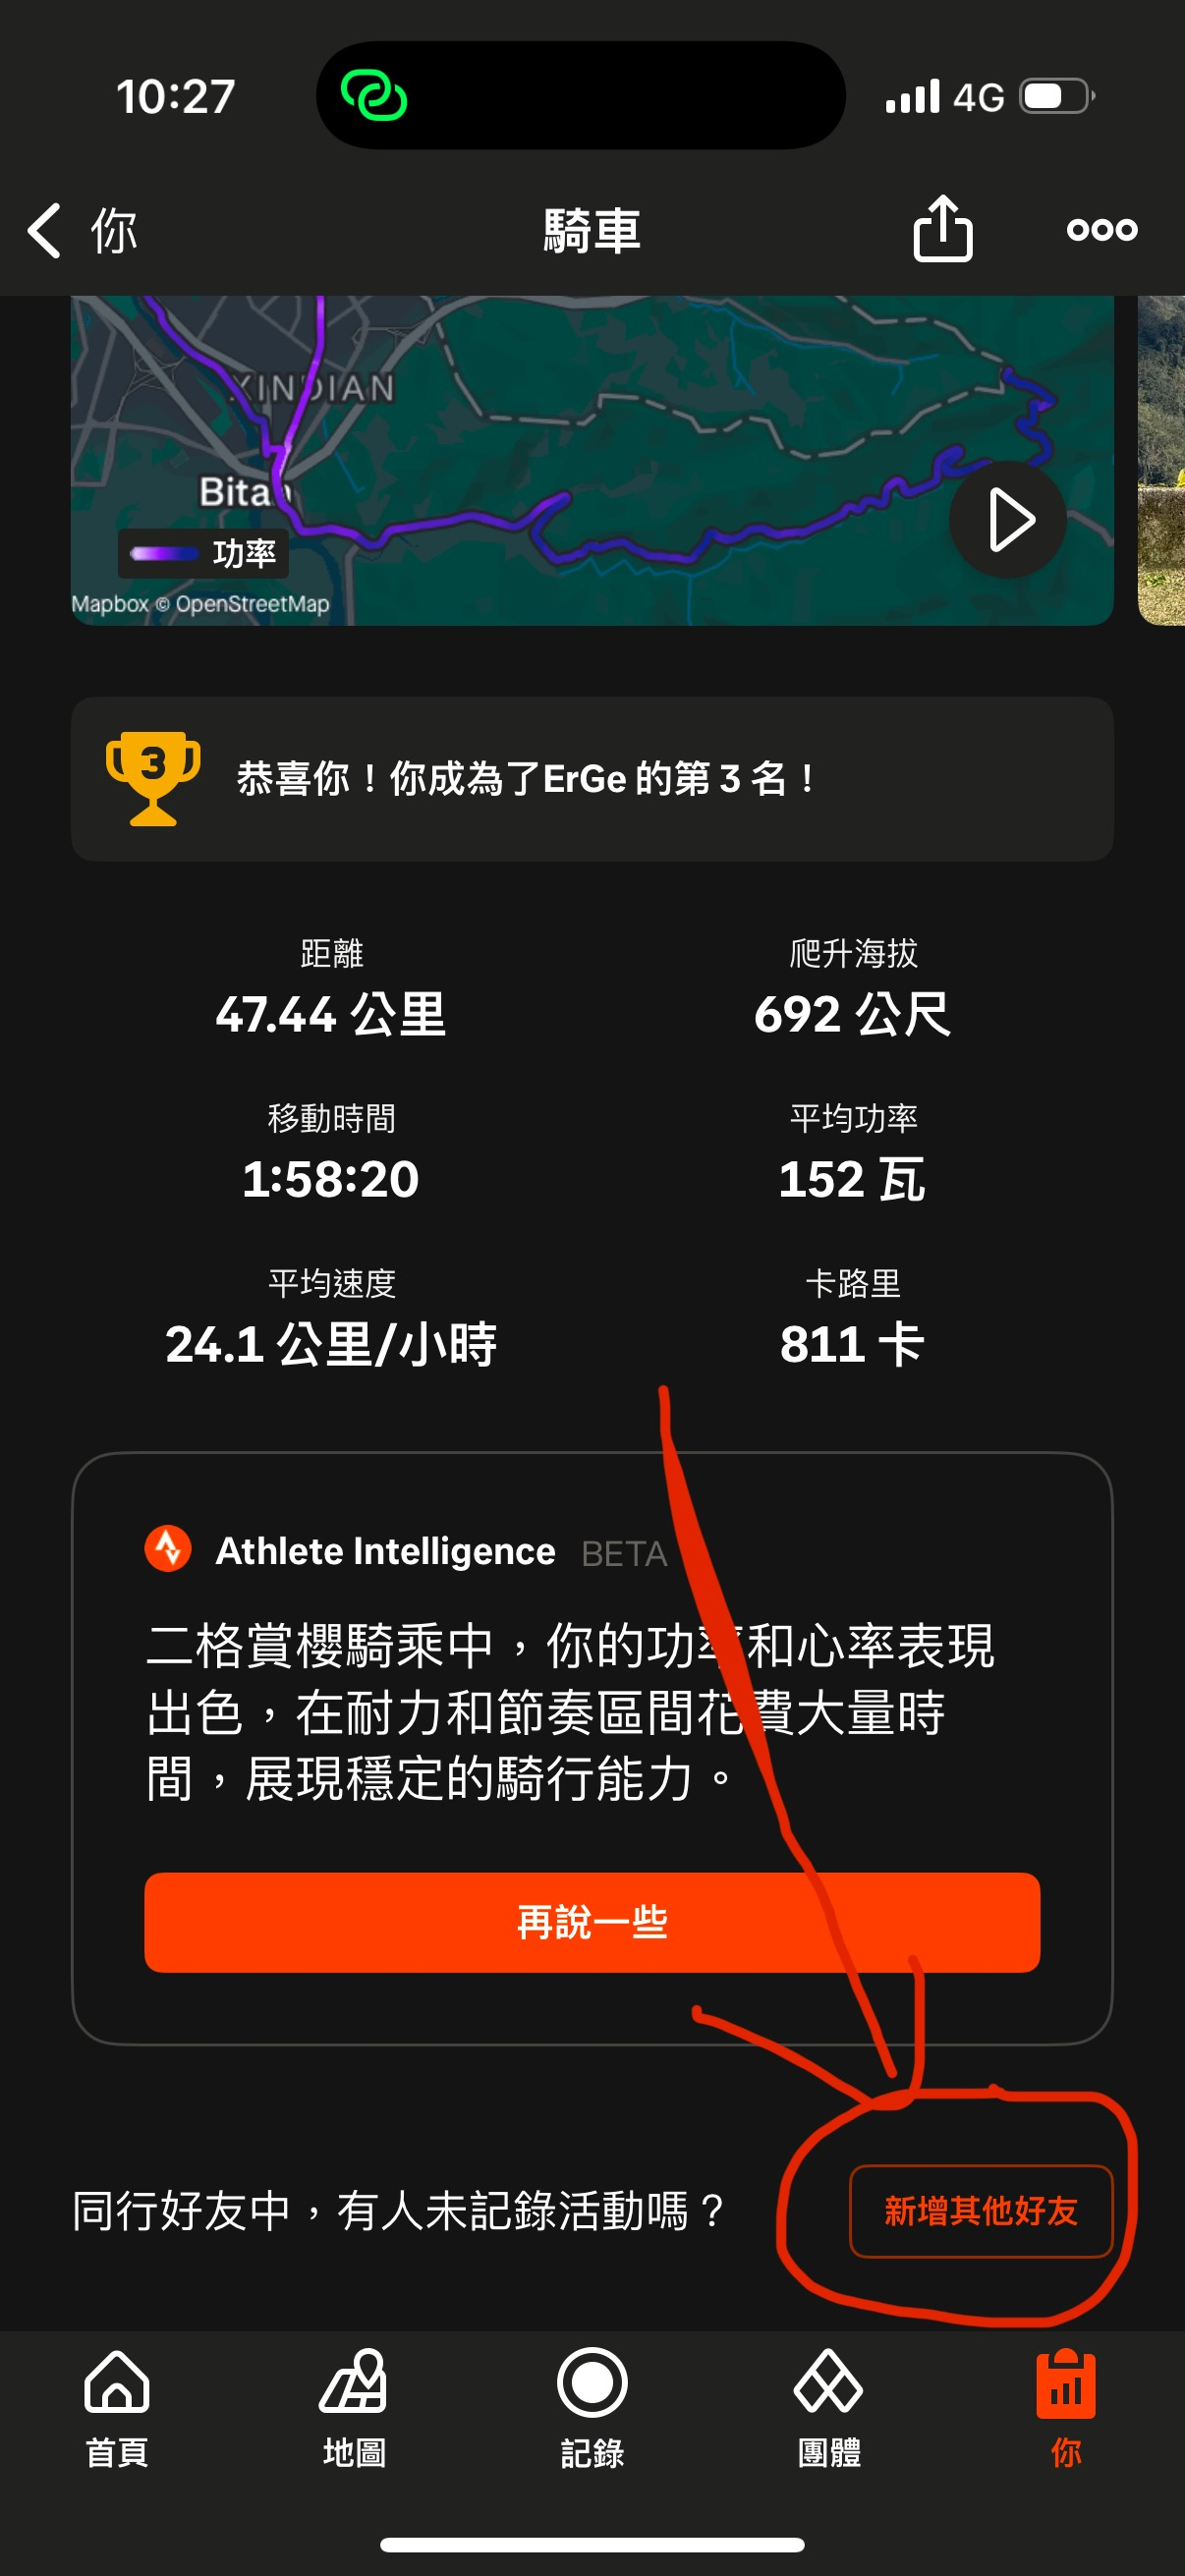
\includegraphics[width=3cm]{rideTogether2.png}
\newpage
\item 如果A在某個活動中有$50\%$以上的時間是在B的某個活動的附近,那 Strava 會在A的活動中說與B一起騎乘
\item 是否一起騎乘並不是對稱的(在數學上的說法是並非等價關係)\\
{\tiny 等價關係是指具有自反性、對稱性、遞移性的二元關係}\\
舉例來說,A的某個活動是跟了B的某個$24$小時的活動的最前面$8$的小時(例如B騎一日台九而A騎一日北花),那在A的活動中會寫跟B一起騎乘,但是在B的活動中不會寫跟A一起騎乘
\end{itemize}
\end{multicols}
\end{frame}

\begin{frame}{尋找活動}
\begin{itemize}
\only<1>{
\begin{multicols}{2}
\item 依照名稱尋找(僅限自己的活動)\\
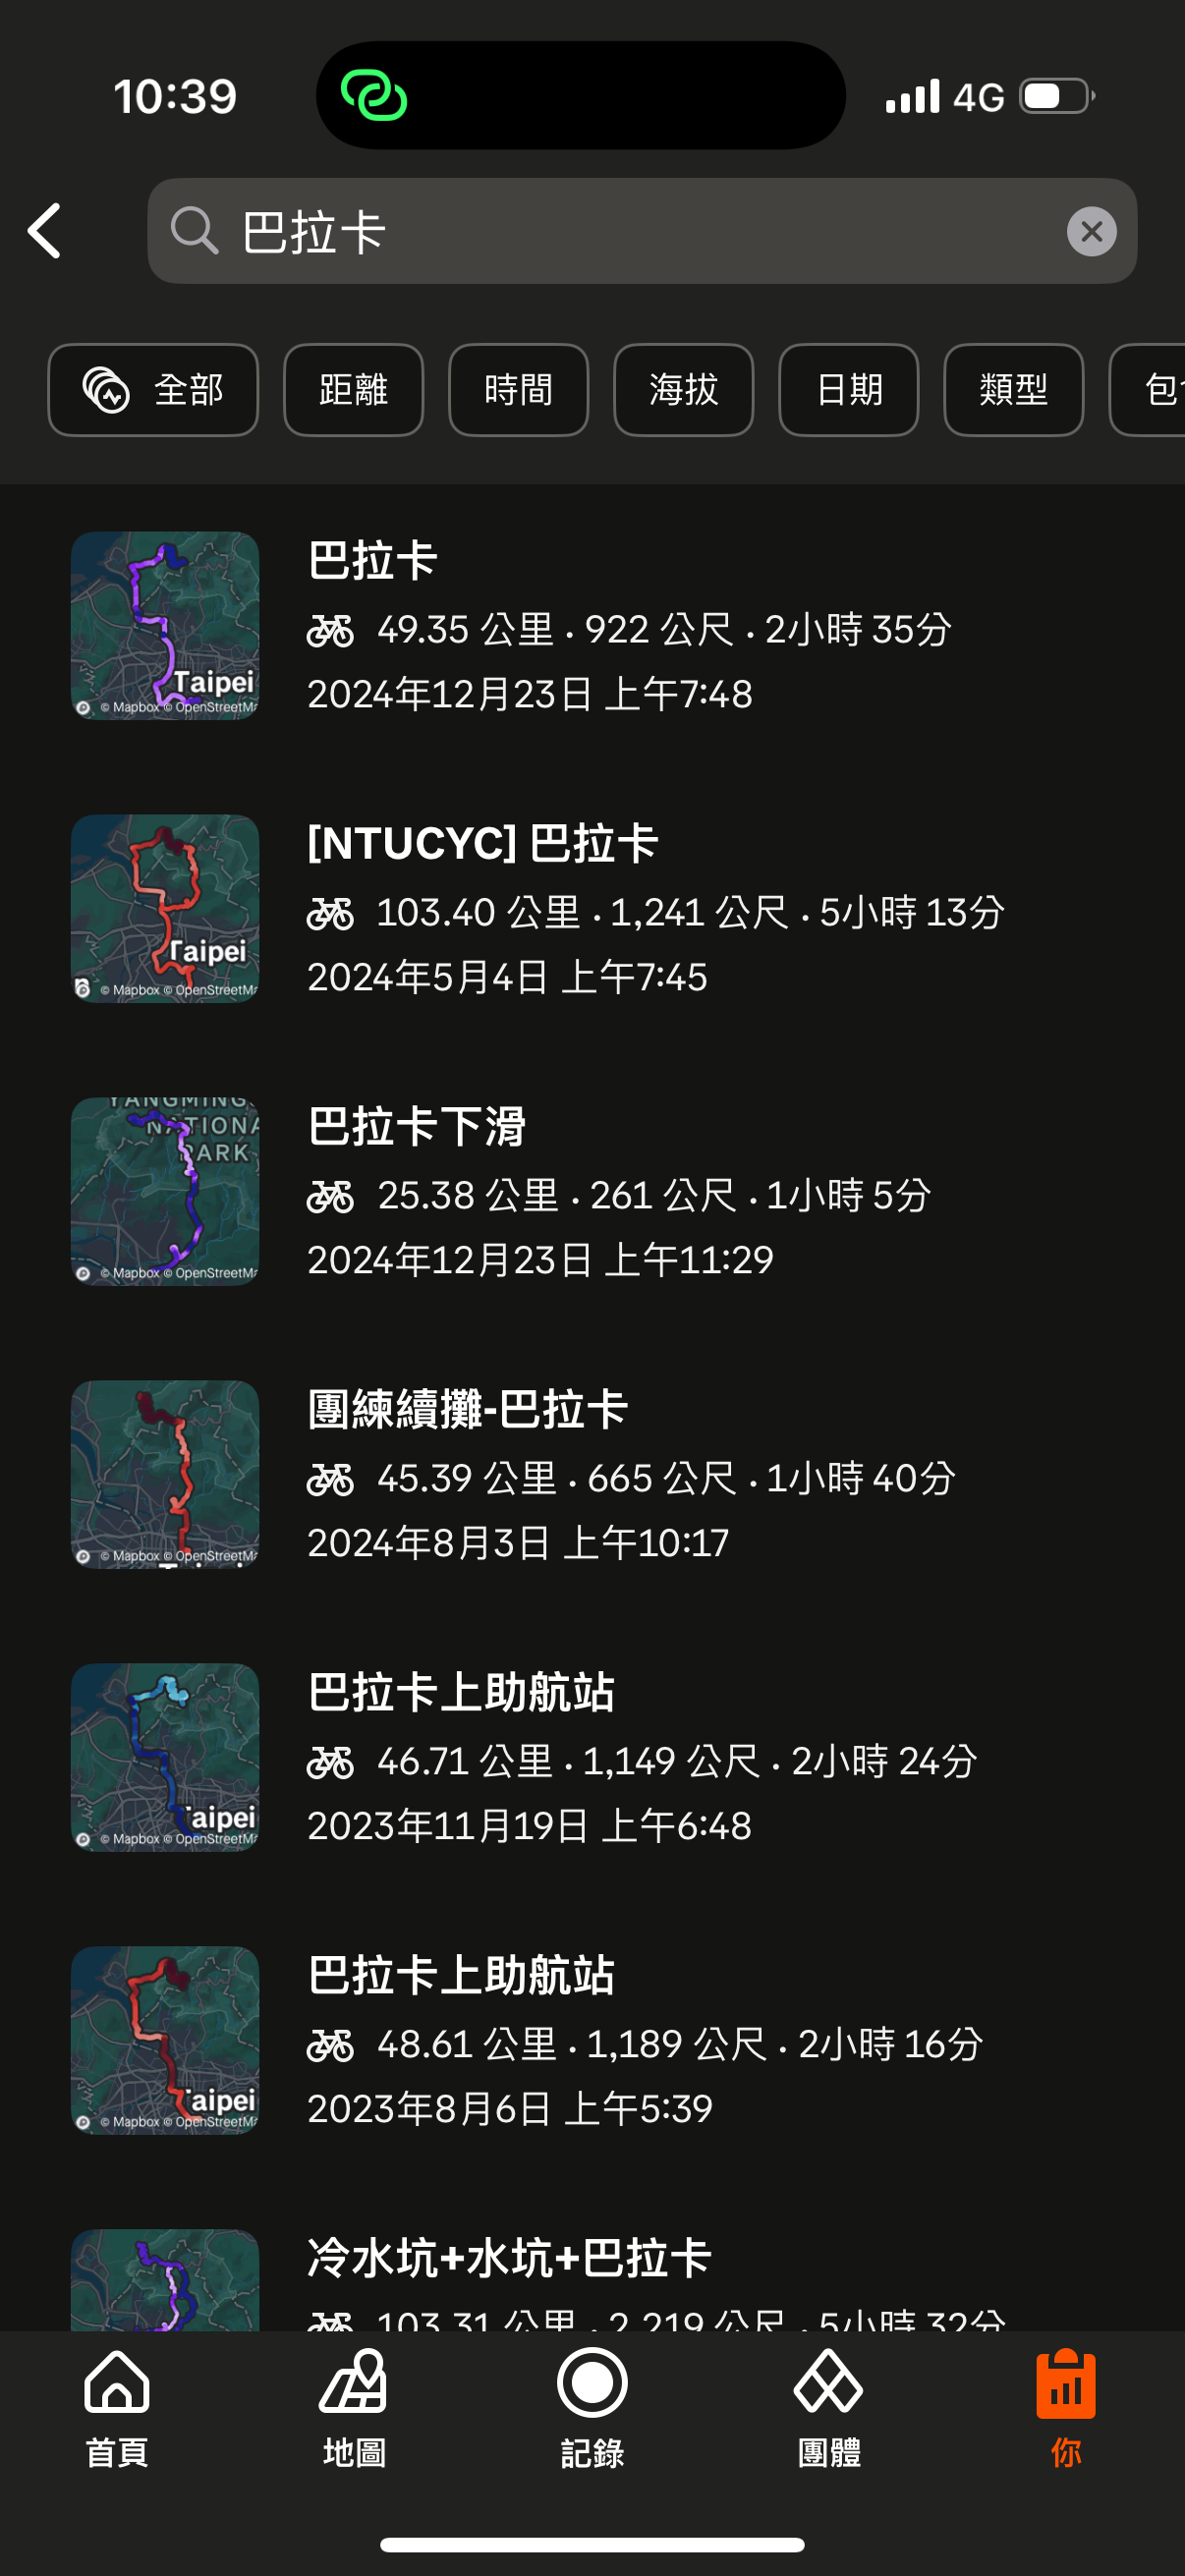
\includegraphics[width=3cm]{getActivityByName.png}
\item 依照名稱尋找別人的活動:需要寫爬蟲\\
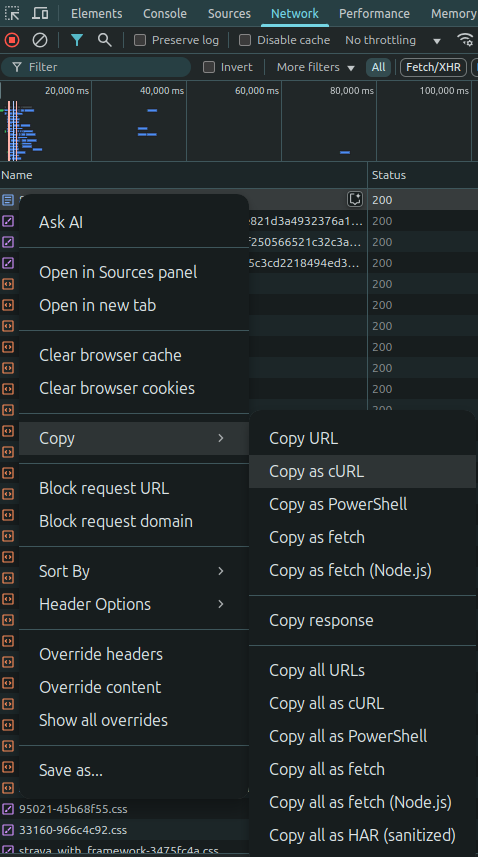
\includegraphics[height=6cm]{crawl.png}
\end{multicols}
}\only<2>{
\begin{multicols}{2}
\item 依照時間尋找(網頁版)\\
\begin{itemize}
\item 自己的:點右上角頭貼,然後點「My Profile」
\item 別人的:左上角搜尋那個人,搜完之後就看到了
\end{itemize}
點你要找的時間對應的那一條,會顯示所有在那一週的活動
\newpage
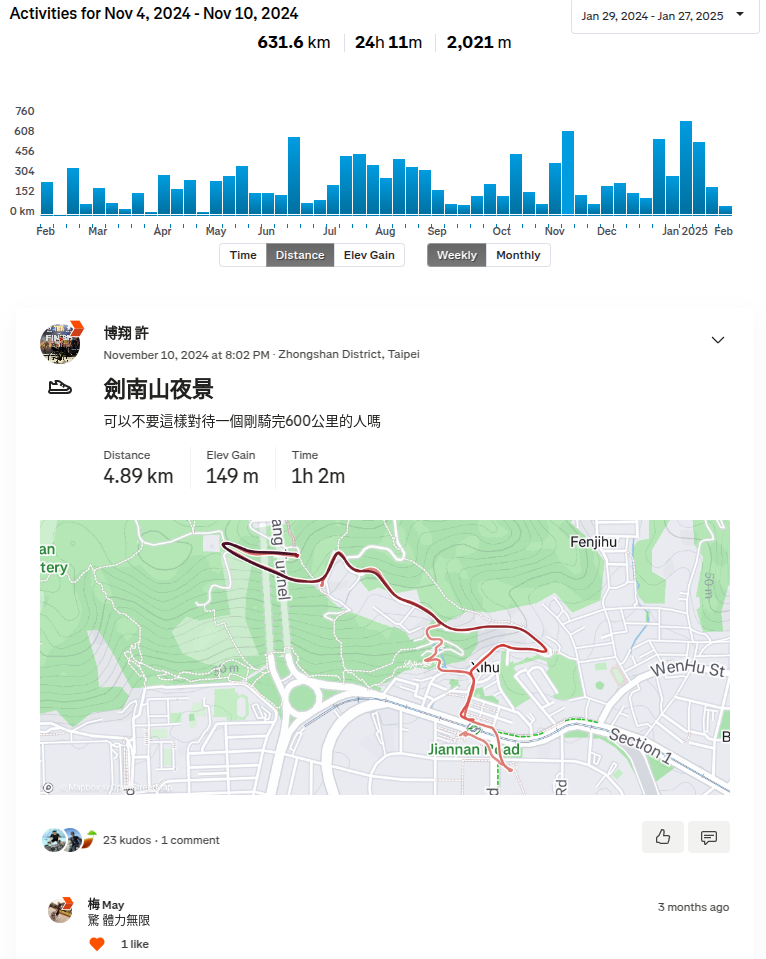
\includegraphics[width=5cm]{getActivityByTime.png}
\end{multicols}
}
\end{itemize}
\end{frame}

\begin{frame}{播放活動}
\begin{itemize}
\item 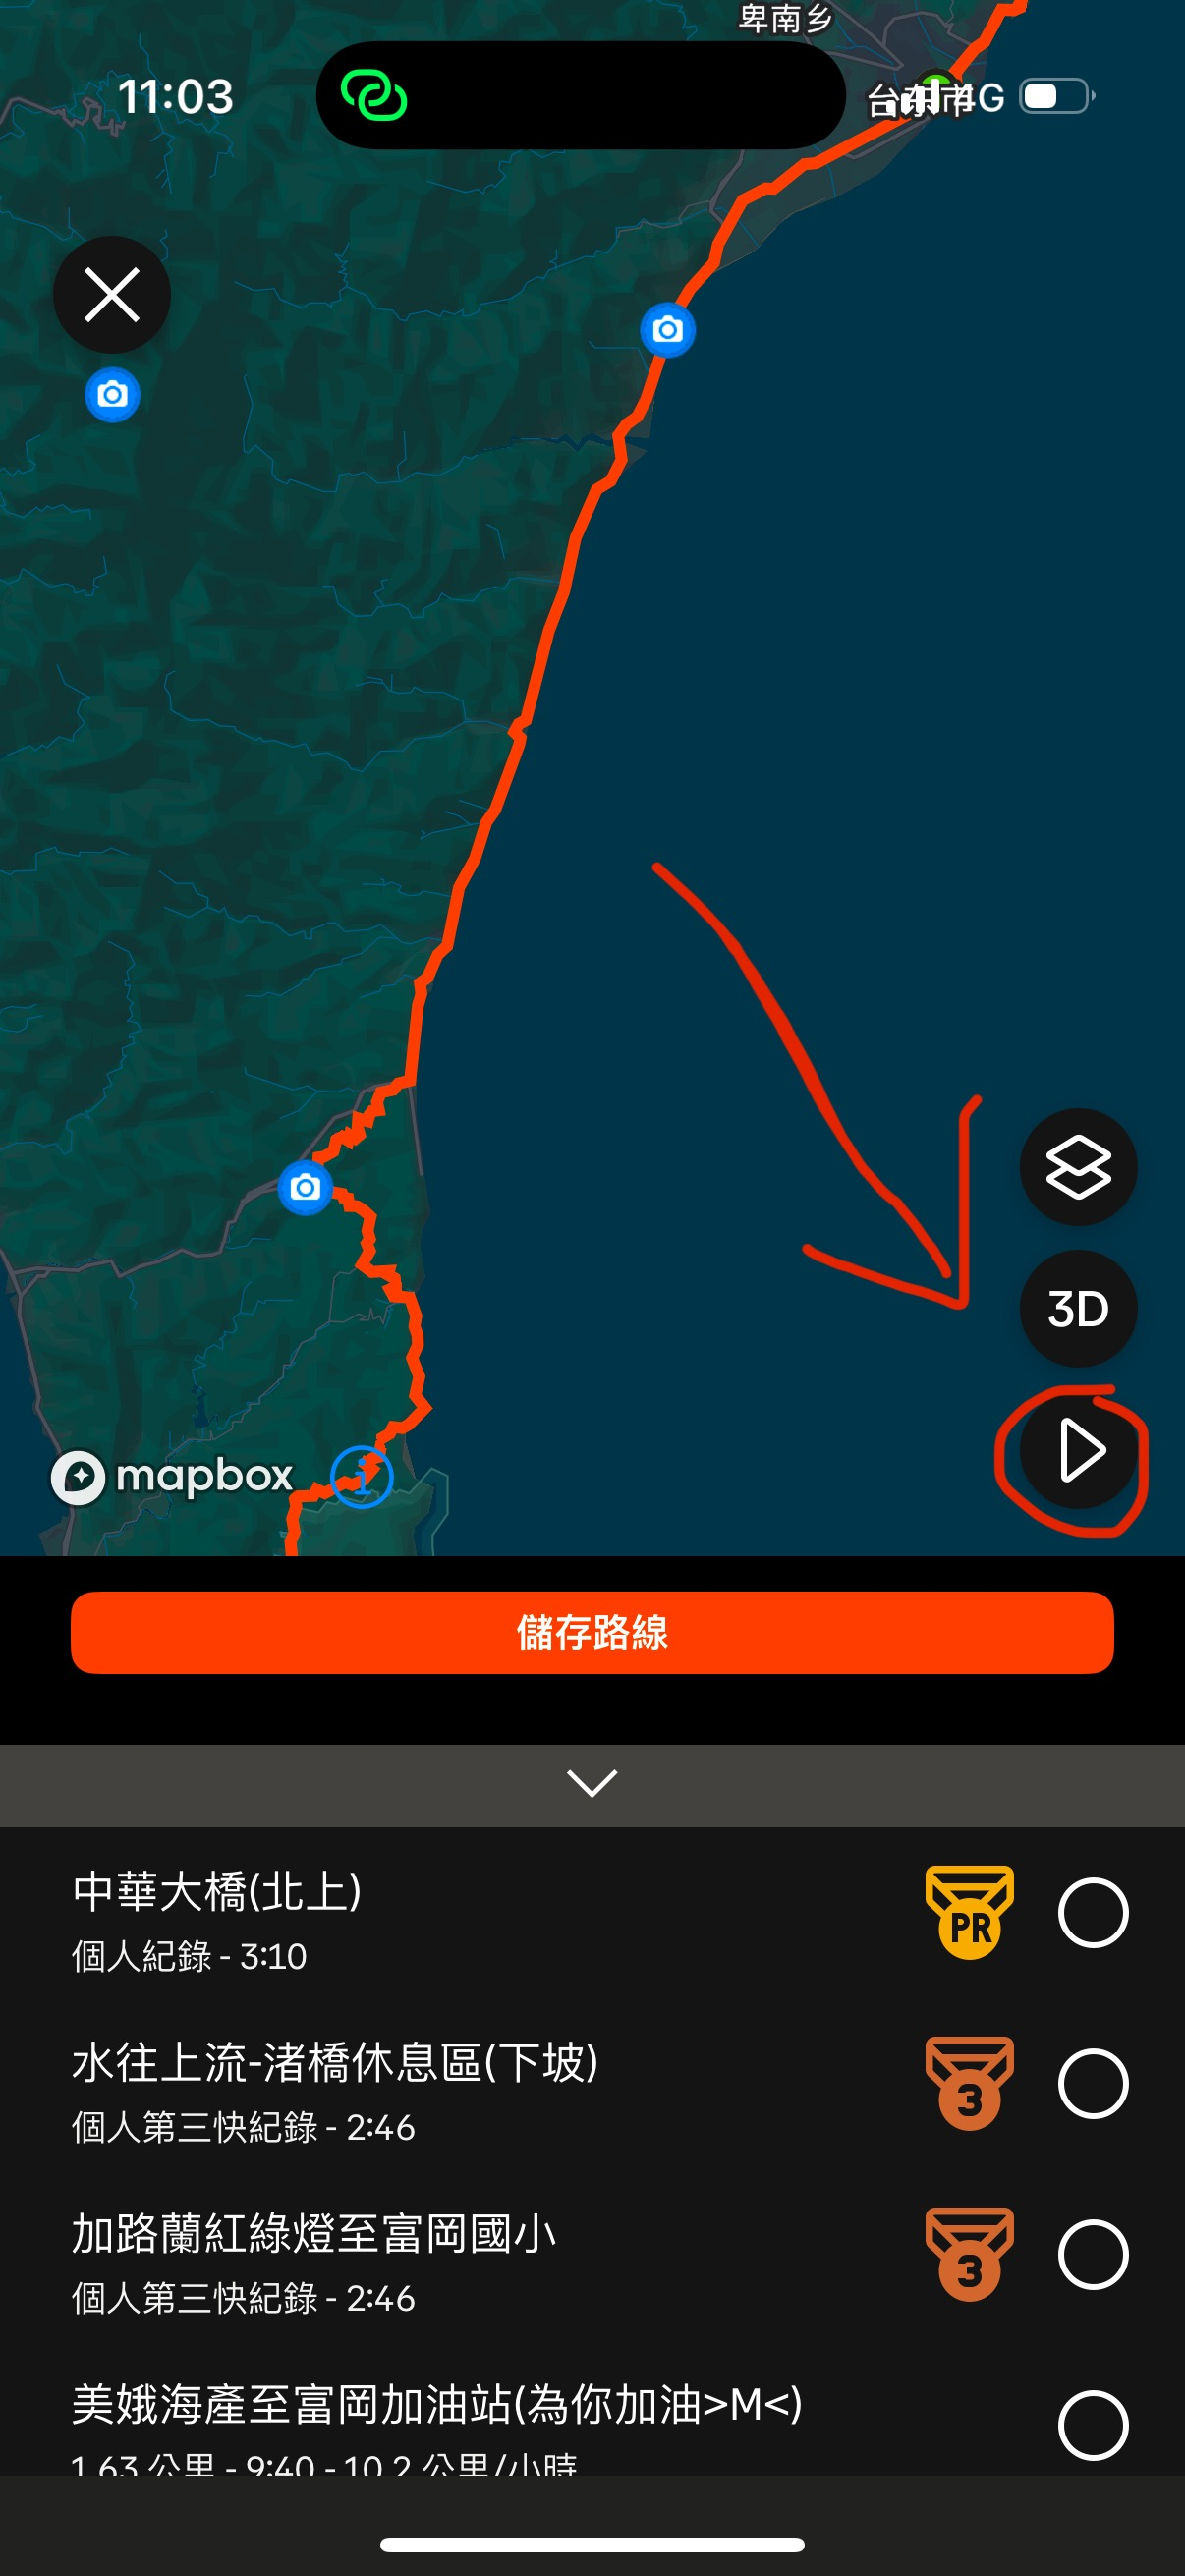
\includegraphics[width=3.2cm]{playActivity.png}
\includegraphics[width=3.2cm]{playActivityWuling.png}
\includegraphics[width=3.2cm]{playActivityTaitung.png}
\includegraphics[width=3.2cm]{playActivityTataka.png}
\end{itemize}
\end{frame}
